%% This is file `elsarticle-template-1-num.tex',
%%
%% Copyright 2009 Elsevier Ltd
%%
%% This file is part of the 'Elsarticle Bundle'.
%% ---------------------------------------------
%%
%% It may be distributed under the conditions of the LaTeX Project Public
%% License, either version 1.2 of this license or (at your option) any
%% later version.  The latest version of this license is in
%%    http://www.latex-project.org/lppl.txt
%% and version 1.2 or later is part of all distributions of LaTeX
%% version 1999/12/01 or later.
%%
%% Template article for Elsevier's document class `elsarticle'
%% with numbered style bibliographic references
%%
%% $Id: elsarticle-template-1-num.tex 149 2009-10-08 05:01:15Z rishi $
%% $URL: http://lenova.river-valley.com/svn/elsbst/trunk/elsarticle-template-1-num.tex $
%%
\documentclass[preprint,12pt]{elsarticle}

%% Use the option review to obtain double line spacing
%% \documentclass[preprint,review,12pt]{elsarticle}

%% Use the options 1p,twocolumn; 3p; 3p,twocolumn; 5p; or 5p,twocolumn
%% for a journal layout:
%% \documentclass[final,1p,times]{elsarticle}
%% \documentclass[final,1p,times,twocolumn]{elsarticle}
%% \documentclass[final,3p,times]{elsarticle}
%% \documentclass[final,3p,times,twocolumn]{elsarticle}
%% \documentclass[final,5p,times]{elsarticle}
%% \documentclass[final,5p,times,twocolumn]{elsarticle}

%% The graphicx package provides the includegraphics command.
\usepackage{graphicx}
%% The amssymb package provides various useful mathematical symbols
\usepackage{amssymb}
%% The amsthm package provides extended theorem environments
\usepackage{amsmath}
\usepackage{amsmath,latexsym} 
\usepackage{mathabx}
\usepackage{url} 

%to see highlighted text and allow subfigures
\usepackage{color,soul,xcolor}
\usepackage{subcaption}
\usepackage{hyperref}

%% The lineno packages adds line numbers. Start line numbering with
%% \begin{linenumbers}, end it with \end{linenumbers}. Or switch it on
%% for the whole article with \linenumbers after \end{frontmatter}.
\usepackage{lineno}

%% natbib.sty is loaded by default. However, natbib options can be
%% provided with \biboptions{...} command. Following options are
%% valid:

%%   round  -  round parentheses are used (default)
%%   square -  square brackets are used   [option]
%%   curly  -  curly braces are used      {option}
%%   angle  -  angle brackets are used    <option>
%%   semicolon  -  multiple citations separated by semi-colon
%%   colon  - same as semicolon, an earlier confusion
%%   comma  -  separated by comma
%%   numbers-  selects numerical citations
%%   super  -  numerical citations as superscripts
%%   sort   -  sorts multiple citations according to order in ref. list
%%   sort&compress   -  like sort, but also compresses numerical citations
%%   compress - compresses without sorting
%%
%% \biboptions{comma,round}

% \biboptions{}

%\journal{Journal Name}
\begin{document}

\begin{frontmatter}

%% Title, authors and addresses

\title{Binary Neutron Star Systems: Analysis of simulated data to understand their evolution}

%% use the tnoteref command within \title for footnotes;
%% use the tnotetext command for the associated footnote;
%% use the fnref command within \author or \address for footnotes;
%% use the fntext command for the associated footnote;
%% use the corref command within \author for corresponding author footnotes;
%% use the cortext command for the associated footnote;
%% use the ead command for the email address,
%% and the form \ead[url] for the home page:
%%
%% \title{Title\tnoteref{label1}}
%% \tnotetext[label1]{}
%% \author{Name\corref{cor1}\fnref{label2}}
%% \ead{email address}
%% \ead[url]{home page}
%% \fntext[label2]{}
%% \cortext[cor1]{}
%% \address{Address\fnref{label3}}
%% \fntext[label3]{}


%% use optional labels to link authors explicitly to addresses:
%% \author[label1,label2]{<author name>}
%% \address[label1]{<address>}
%% \address[label2]{<address>}

\author{Andrea Nicolai, Camilla Quaglia, Sandeep Kumar Shekhar and Walter Zigliotto}

\address{Department of Physics and Astronomy \\ Università degli Studi di Padova \\via 8 Febbraio 1848, 2, 35122 Padova PD}

\begin{abstract}
This work aims to understand the formation of the sources of gravitational waves, in particular the formation of binary neutron stars. Data used is simulated by MOBSE. The analysis considers binary neutron stars systems that merge within a Hubble time. Besides, this work gives an overview about the nature of their physical properties such as masses of progenitors, mass of Compact Objects formed, type and number of Common Envelopes and finally delay time densities for varying metallicities and $fMT$s.  
\end{abstract}

\begin{keyword}
Binary Neutron Stars \sep Data \sep Compact Objects \sep Common Envelopes \sep metallicities \sep $fMT$.
%% keywords here, in the form: keyword \sep keyword

%% MSC codes here, in the form: \MSC code \sep code
%% or \MSC[2008] code \sep code (2000 is the default)

\end{keyword}

\end{frontmatter}

%%
%% Start line numbering here if you want
%%
%\linenumbers

%% main text
\section{Introduction}
\label{S:1}
The Einstein's general theory of relativity revolutionized the field of physics\citep{Einstein:1916}. The theory relates the curvature in space-time with the energy of the object. The Einstein equation is given as:
\begin{equation}
R_{\alpha\beta}-\frac{R}{2}g_{\alpha\beta} = \frac{8\pi G}{c^4}T_{\alpha\beta}    
\end{equation}
Where $R_{\alpha\beta}$ is the Ricci tensor, $R$ is the Ricci scalar, $g_{\alpha\beta}$ is the metric and $T_{\alpha\beta}$ is the stress energy tensor. The linearised field equations (expanded as a perturbation of the flat space-time Lorentz metric) has the form of a relativistic wave equation with the space-time perturbation propagating as a wave (so-called ripples of geometry) moving at the speed of light. The propagating field is a second order tensor field which in vacuum has the form $\Box^2 \phi_{\alpha \beta}=0$\citep{Einstein:1918} ($\Box$ is the d'alembertian operator), i.e.,
\begin{equation}
\frac{\partial^2 \phi_{\alpha \beta}}{\partial t^2}-\frac{1}{c^2}\nabla^2\phi_{\alpha \beta} = 0
\end{equation}

Where $\phi$ is the scalar field, and $\nabla$ is the Laplace operator. Gravitational waves were detected in the year 2015\citep{Abbott:2016}. The waves were the result of the merger of Binary Black Holes (BBH). Several events have been detected in the recent past\citep{Abbott:2017, Abbott:2017b, Abbott:2017c}. Previously cited references are the waves from the BBH. Our work involves the evolution of Binary Neutron Stars (BNS). The coalescence of BNS observed in the year 2017\citep{Abbott:2017d} and the electromagnetic counterpart observed as short Gamma-Ray Burst (GRB), with a delay of $+ 1.74 \pm 0.05$s\citep{Abbott:2017e, Goldstein:2017}. Jocelyn Bell Burnell and Antony Hewish discovered pulsars in 1967\citep{Hewish:1968}, which later identified as rapidly rotating NS. NS are astronomical objects with densities roughly of the order of $10^{17}-10^{18} kg m^{-3}$\citep{Hartle:1977, Goldman:1989}, roughly $10^8$ times higher than that of a white dwarf. The NS's that exist in nature found to be $<3M_{\odot}$. There has been a lot of development in the nuclear theory describing the internal constituents of the NS in recent years. The constraints placed on the Equation of State (EoS) of NS determines the mass of the NS. The maximum mass of NS is altogether a new topic of study, the constraints involving the quarks\citep{Weber:2006}, f(R) gravity\citep{Capozziello:2016}, presence of dark matter particles\citep{KUMAR:2020}. LIGO-VIRGO collaborations have also involved in understanding the nature of these compact binaries.\\

Our work involves understanding the binary progenitor stars evolution resulting in the formation of BNS. We observe more than $55\%$ of the stars in our galaxy are binary and multiple stars\citep{Sana:2012}. The progenitor stars that form NS are in the mass range of $\sim 9-20 M_{\odot}$. All-stars undergo the main sequence phase, characterized by core hydrogen burning, and spend $90\%$ of their lifetime in the hydrogen-burning phase. The hydrogen-burning timescale for a $13M_\odot, 15M_\odot, 20M_\odot$ star is  around $13, 11, 8$ million years respectively\citep{Woosley:2002}. One of the salient features of stellar evolution is the mass loss. Stars lose mass at all evolutionary stages, including the main sequence. The rates of mass loss vary, however, over a wide range. Thus, the mass-loss rate is so slow as to have a discernible effect on the stellar mass. The solar wind, for example, removes the mass from the Sun at a rate of $\sim 10^{-14}M_\odot yr^{-1}$\citep{Dina:2009}. 

\subsubsection{\textbf{Mass Transfer}}
In the binary systems, the mass transfer occurs between the stars by three prominent mechanisms:\newline
\begin{itemize}
    \item Wind transfer
    \item Roche Lobe Overflow (RLO)
    \item Common Envelope (CE)
\end{itemize}

\begin{figure}[htp]
    \centering
    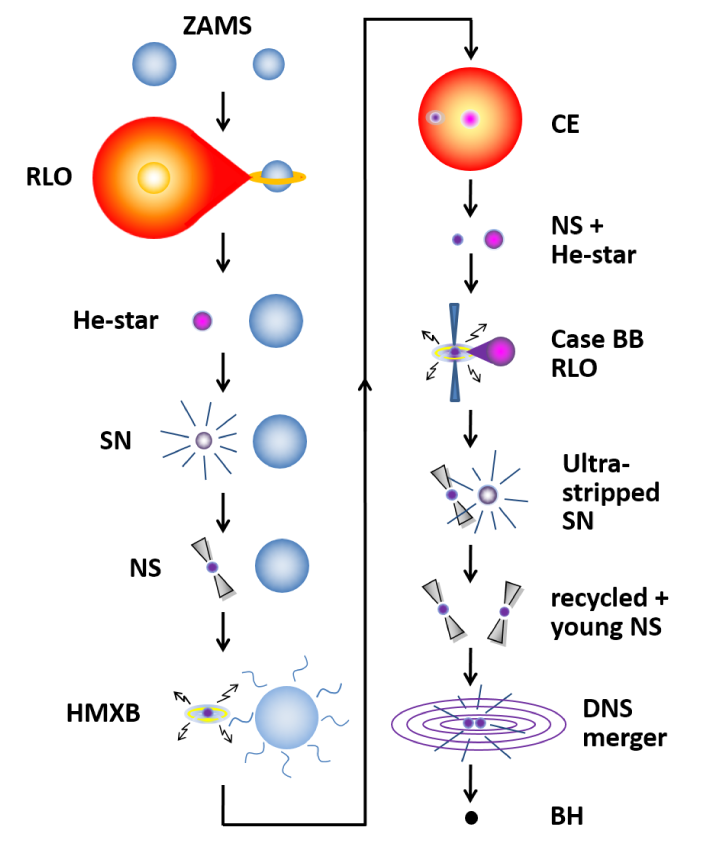
\includegraphics[width=0.5\textwidth]{Images/x1.png}
    \caption{A typical formation channel of the BNS\citep{Tauris:2017}. ZAMS:Zero Age Man Sequence, RLO: Roche Lobe Overflow, He-star: Helium-star, SN: Supernova, HMXB: High Mass X-Ray Binary, CE: Common Envelope, DNS: Double Neutron Star.}
    \label{img:Formation channel DNS}
\end{figure}

\subsubsubsection{\textbf{Wind transfer}}\newline
The primary progenitor (biggest of the two) loses mass by stellar winds. The stellar winds in very massive stars are due to the coupling through resonant metal lines, hence making it explicitly dependent on metallicity. The secondary accretes the mass lost as stellar winds from the primary and given as\citep{Bondi:1944}:

\begin{equation}
    \frac{|\Dot{M}_{2A}|}{|\Dot{M}_{1W}|} \propto \Big(\frac{v_{orb}}{v_W}\Big)^4
\end{equation}

Where $\Dot{M}_{2A}$ is the mass accreted by the secondary, $\Dot{M}_{1W}$ represents the mass loss due to the stellar winds from the primary and $v_W$ is the wind velocity. This model is an inefficient way to describe mass transfer. There has been a significant development to find an ideal model for mass loss through stellar winds.\newline


\subsubsubsection{\textbf{Roche Lobe Overflow}}\newline
The BNS formation involves the primary progenitor exhausting hydrogen burning in the core and the outer layers of the star to expand (Red Giant Phase). The secondary progenitor accretes the outer expanded layers of the primary star, leading to a mass gain. This process results in a Roche-Lobe Overflow (RLO). There exist equipotential points in a binary system and are called Lagrangian points (L1, L2, L3, L4). These Lagrangian points separate the lobes. When the primary star's outer layer radius becomes greater or equal to the innermost Lagrangian point (L1), the mass transfer occurs to the secondary star. This phenomenon is known as Roche lobe overflow. The effective radius ($R_L$) is given as\citep{Eggleton:2006}:

\begin{equation}
    \frac{R_L}{a}\approx\frac{0.49q^\frac{2}{3}}{0.6q^\frac{2}{3}+ln(1+q^\frac{1}{3})}
\end{equation}

Where $q=m1/m2$ and $a$ is the orbital separation. RLO continues if $q>1$ and i.e., $m1>m2$. During this span, the orbital separation shrinks between the stars. Once the masses are equal and $m1<m2$ the orbital separation and donor's Roche lobe increase.\newline


\subsubsubsection{\textbf{Common Envelope}}\newline
The Common Envelope usually forms when one of the stars is a compact object in a binary star system, and the other begins to expand rapidly\citep{Iben:1993}. The donor star will start mass transfer when it overfills its Roche lobe. As a consequence of this, the orbit shrinks further, causing it to overflow the Roche lobe even more, which accelerates the mass transfer, causing the orbit to shrink even faster and the donor to expand more. This leads to the runaway process of dynamically unstable mass transfer. In some case, the receiving star is unable to accept all material, which leads to the formation of a Common Envelope engulfing the companion star\citep{Ivanova:2013}.\newline


Fig.\ref{img:Formation channel DNS} depicts a summary of typical BNS formation. The binary progenitors are in the ZAMS phase. One of the stars exhaust hydrogen burning in the core and expand the outer layers filling the Roche lobes. The secondary star accretes matter from the primary. The primary explodes as a supernova, and a compact core left as a remnant. The NS accretes the mass from secondary, and emit X-rays. The secondary's outer envelope encloses the NS. The mass is accreted by the NS. If the Common Envelope ejects, then the binary system retains. The secondary star undergoes supernova and leaves behind NS. The primary and the secondary NS form a tight binary and finally merge to either NS or BH.


\subsubsection{\textbf{fMT}}
fMT is a parameter that determines the mass transfer efficiency. It plays a prominent role in deciding the fate of the binaries. If the accretor is a non-degenerate star, then fMT is represented as:

\begin{equation}
  \Dot{M}_{accretor}=fMT(|\Dot{M}_{donor}|)
\end{equation}

In case the accretor is a compact object, then fMT is:

\begin{equation}
  \Dot{M}_{accretor}= min(|\Dot{M}_{donor}|)(|\Dot{M}_{Edd}|)
\end{equation}


\section{Methods}

The focus of our study is on the statistical analysis of a large number of BNS systems through simulated data. This analysis is done using Python 3.7.7, in particular, NumPy 1.18.1 and Pandas 1.0.3 libraries. The data stored in an external server has been accessed remotely by the means of a VPN.\\

MOBSE (Massive Objects in Binary Stellar Evolution) is a simulated population synthesis code, developed by Hurley as BSE\citep{Hurley:2002} and upgraded by Giacobbo, Mapelli, and Spera\citep{Giacobbo:2017}, to investigate the evolution of binary stellar systems. In particular, MOBSE takes into account of metallicity-dependent prescriptions for stellar winds, the dependency of mass loss on the electron-scattering Eddington factor of the star, and new solutions for core-collapse SN. \\

For this analysis, the dataset, generated through MOBSE, consists of about a billion binary systems of isolated massive binaries over a Hubble time. The prominent features such as metallicity ($Z$), Roche lobe mass transfer efficiency ($fMT$), and the parameter $\alpha$ (energy removal efficiency) set as:

\begin{itemize}
    \item $Z$ : 0.02, 0.016, 0.012, 0.008, 0.006, 0.004, 0.002, 0.0016, 0.0012, 0.0008, 0.0004 and 0.0002.
    \item $fMT$: 1, 0.7, 0.5, 0.4, 0.3, 0.2 and 0.1.
    \item $\alpha$ : 5.
\end{itemize}
Furthermore, data is collected into 5 chunks for computing optimization. According to them, directories are split in a tree structure (Fig.\ref{img:Mobsediagram}), where
each chunks contains the following files: $COB.out$, $CO.out$, $evol\_mergers.out$, $failed\_systems.out$, $input$, $mergers.out$, $params.out$ and $src$. 

\begin{figure}[htp]
\centering
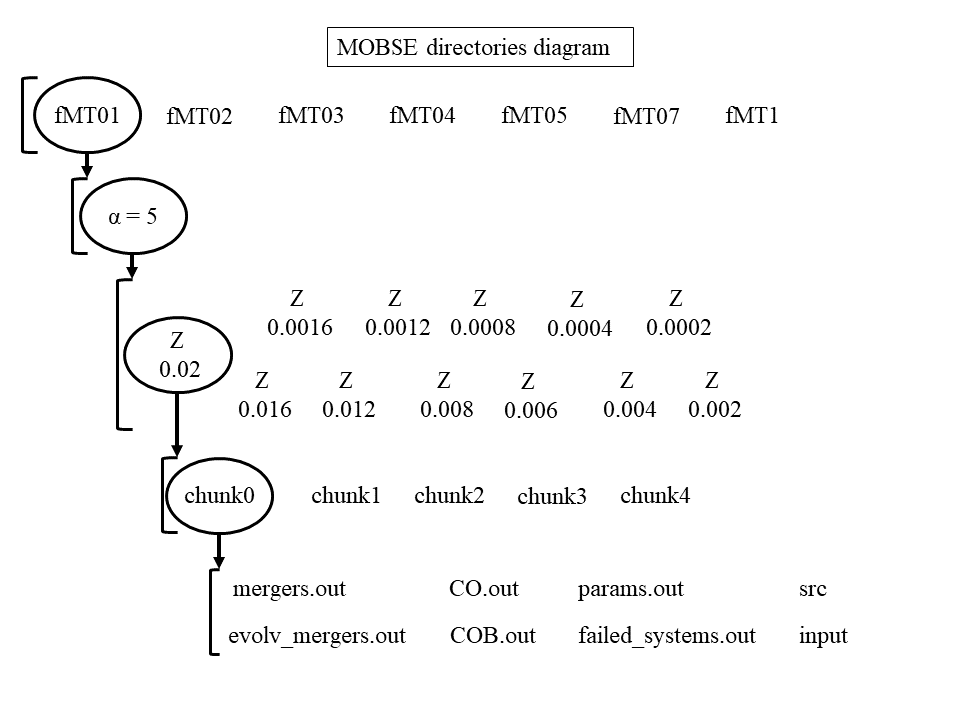
\includegraphics[width = 0.7\textwidth]{Images/MOBSE_diagram.png}
\caption[Methods]{Schematic representation of block directories.}
\label{img:Mobsediagram}
\end{figure}

Nevertheless, the study concentrates on three of them:

\begin{itemize}
    \item $mergers.out$: Information on compact object binaries that merge in a Hubble time.
    \item $evolv\_mergers.out$: Information on each binary system evolution (e.g. Fig.\ref{img:3comenvtime}).
    \item $COB.out$: The output of all compact objects that form.
\end{itemize}

Moreover, the values of mass, luminosity, and radius are expressed in solar units, while the time expressed is in $Myr$ units. Each of the aforementioned datasets includes many parameters. The main parameters taken into account are:
\begin{itemize}
    \item $ID$: Identification number of the binary system.
    \item $k1$, $k2$: Type of the star. The algorithm's stellar types correspond to the evolutionary phases sketch by the rapid SSE (Single Star Evolution) code\citep{Hurley:2002}.
    \item $m_1$, $m_2$: Mass of the star, where $m_1$ is identified as the star coming from the most massive progenitor. 
    \item $t\_step$: The current time of the system.
    \item $label$: Information on the current status of the binary system.
    \item $sep$: The current semi-major axis separation.
\end{itemize}
\begin{figure}[h!]
\centering
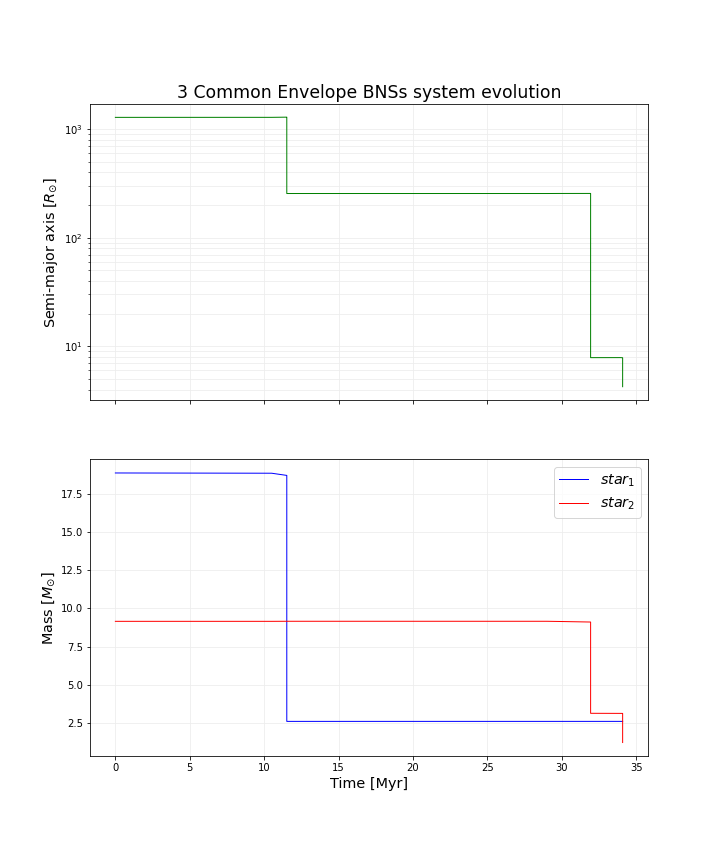
\includegraphics[width = 0.7\textwidth]{Images/3_COMENV_EVOLV.png}
\caption[Methods]{Common envelope time evolution system.}
\label{img:3comenvtime}
\end{figure}

\newpage
\section{Results}

Binary compact object systems may or may not merge within a Hubble time. The analyzed data takes account of both cases. We can count the number of mergers, normalized to the total number of binary systems generated by MOBSE simulation. Generally, for higher values of fMT, we have a lower fraction of systems that merge, although for higher metallicities this trend reverses as seen on the left side of Fig.\ref{img:merging_vs_Z}. This occurs in a flex point, which is around $Z \sim 0.006 $. Moreover, a local minimum is observed around $Z \sim 0.0015$.\\


\begin{figure}[ht]
    \centering
    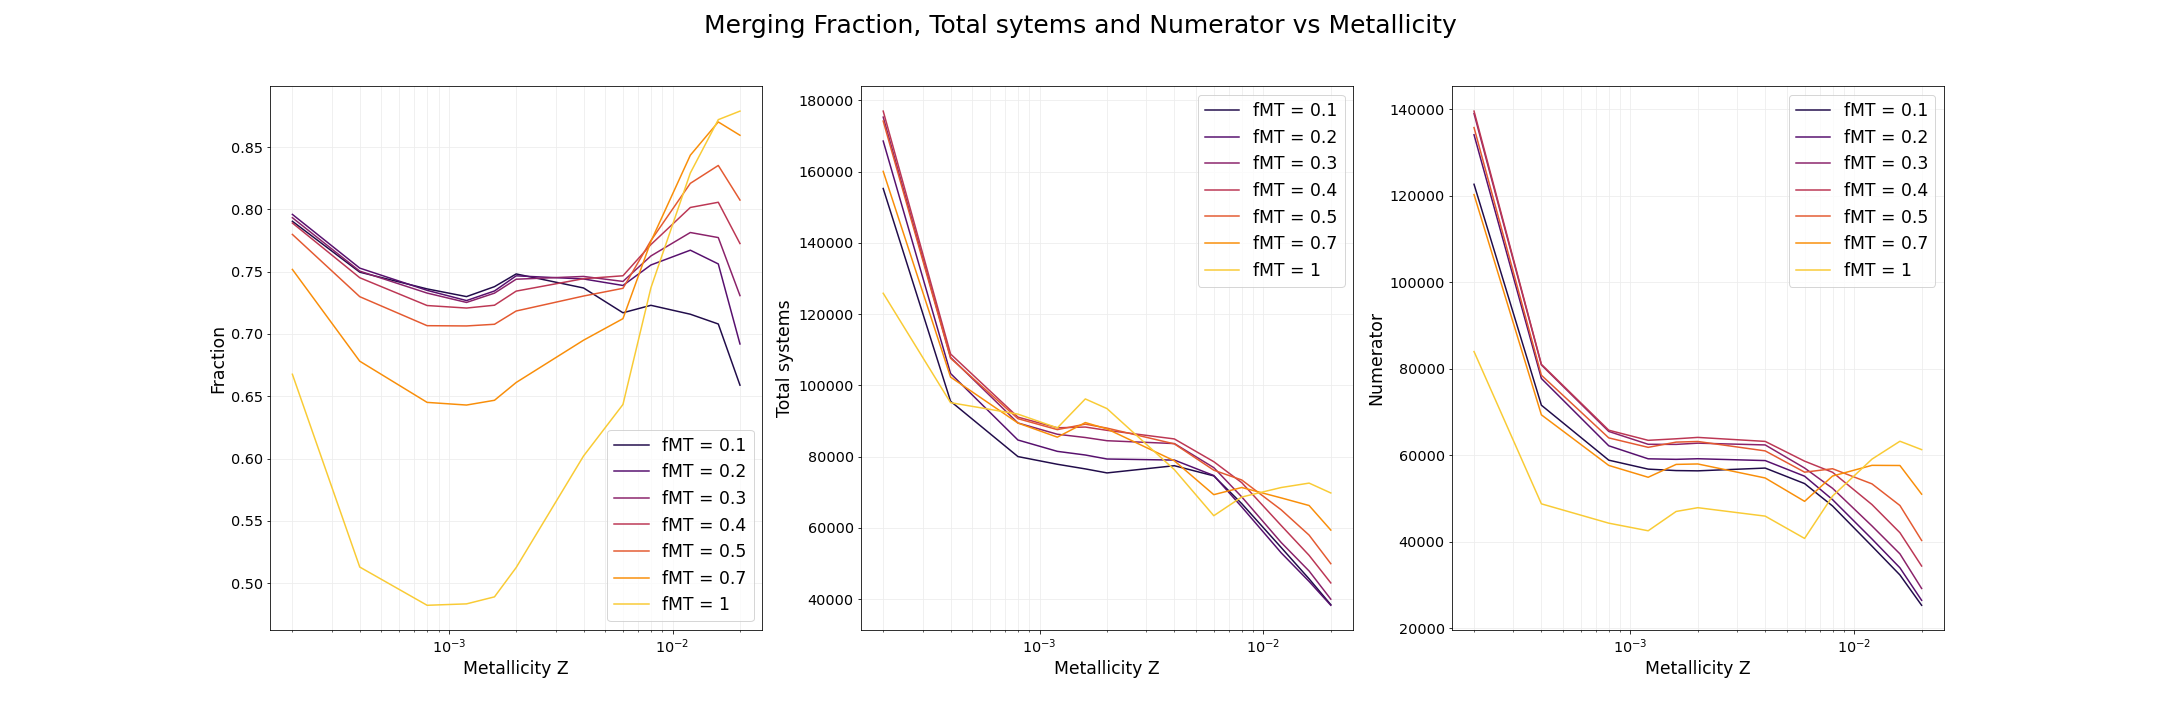
\includegraphics[width=1\textwidth]{Images/total_numerator_fraction (1).png}
    \caption{Left: Fraction of merging systems with respect to the total number. Centre: Total number of systems. Right: Number of merging systems.}
    \label{img:merging_vs_Z}
\end{figure}

To understand the process that leads to a low merging system at $fMT$ = 1 and low $Z$, we assume that the number of BNS is almost the same for all the fMT's, as shown in the Fig.\ref{img:merging_vs_Z}(middle plot). On the other hand, when $fMT$ is very low, binary star systems tend to evolve into BNS. For higher $fMT$ value, the probability for binary star systems to end up as BBH is high. In fact, with low $fMT$, a smaller fraction of the mass loss by the more massive primary star is accreted by the secondary star, thereby the primary ends up as a NS. An efficient mass transfer from the primary to the secondary will result in a latter becoming a BH. Therefore, with a high $fMT$, one can expect a higher probability for a NSBH formation. Also, at $Z \sim 10^{-3}$, the theory of stellar evolution highlights the stellar radii to be comparatively large than at other values of metallicity, especially during the red giant phase. At high metallicities (e.g., solar metallicity), the system loses mass efficiently due to stellar winds. Therefore, hinder the star to have a larger radius. On the contrary, for lower metallicity, the star is compact compared to the intermediate metallicity. This is primarily because of the higher temperature in the core, enabling it to ``burn" a higher amount of fuel and end its life relatively early without losing much mass. At $Z \sim 10^{-3}$, the stars have a striking balance between the percentage of metals and the mass loss. There are several constraints involved in the formation of BNS based on the distance between the binaries. If the progenitor binaries are too close, during the CE phase, the binaries might merge, leaving a massive star or a BH, because of the large radii of the stars. In case the binaries are too far away, we do not expect them to merge in the Hubble time.

\subsection{\textbf{Merging System}}
Our analysis focuses on the systems that merge within a Hubble time by the emission of gravitational waves. Further, we shall consider the ones that are done swiftly without error (included in a specific database). Furthermore, only systems that end up as BNS systems are chosen.

\subsubsection{\textbf{Compact Objects Binary Masses}}

The Fig.\ref{img:ZAMS_vs_NS} highlights the different mass variation between the total non-conservative and strictly conservative systems. 
For $fMT = 0.1$ the massive progenitors are viable. This is because the largest star loses considerably more mass, which is not accreted by the secondary. For such instance, the secondary star is likely to evolve into a NS rather than a BH.
With $fMT = 1$ the $\Delta m_2$ systems are generally shifted at lower side. We expect lower mass second progenitors to be able to form neutron stars because the mass transfer from the massive progenitors is more efficient (during the red giant phase). Furthermore, with a high value of $fMT$, some BNS mergers are lost. Currently, we do not have a good understanding of it. To conclude, Fig.\ref{img:ZAMS_vs_NS} shows that it is possible to end up forming NSs, from massive progenitors ($15 - 25M_{\odot}$).

\begin{figure}[hb]
    \centering
    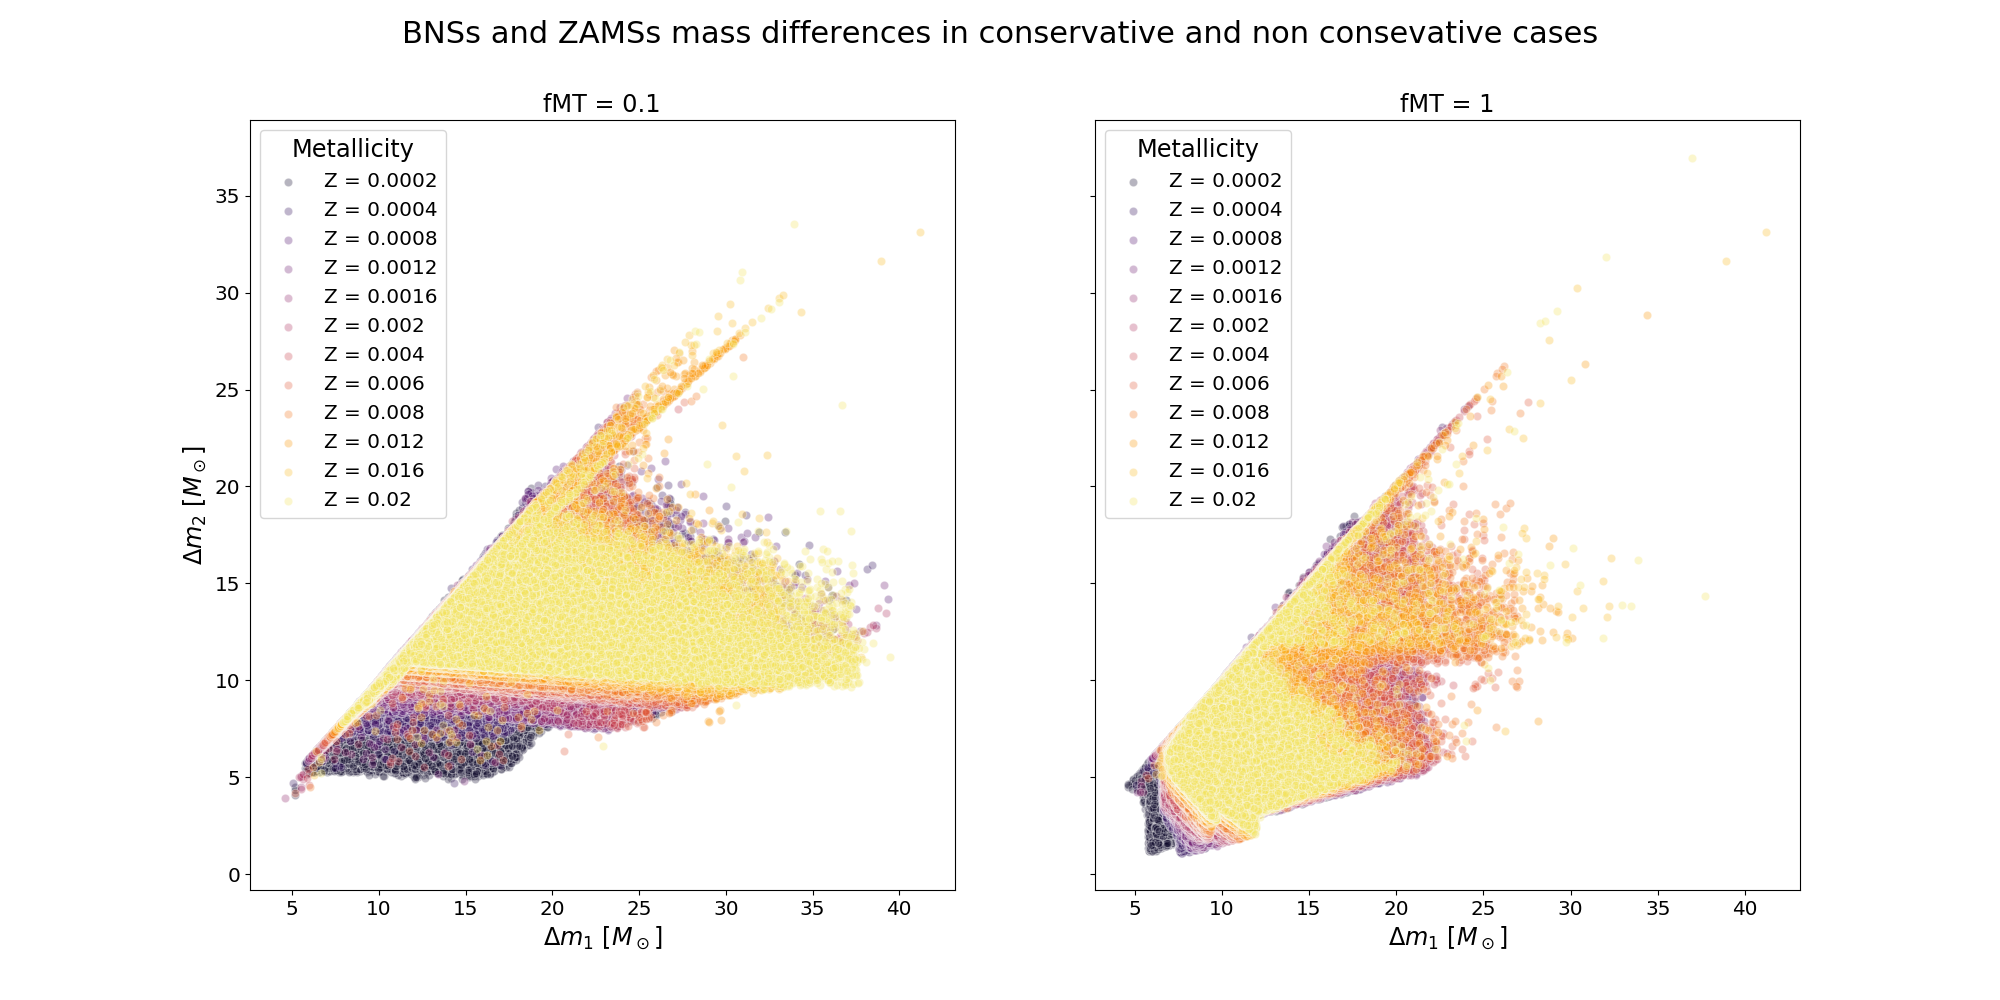
\includegraphics[width=1\textwidth]{Images/ZAMS_vs_BNSs.png}
    \caption{Difference between progenitor's mass and and the NS's mass. On the left fMT = 0.1 and on the right fMT = 1.}
    \label{img:ZAMS_vs_NS}
\end{figure}

The normalized histograms of masses for the two Compact Objects (CO) that form the binary are obtained, for varying $Z$ and fMT, where the primary is more massive than the secondary, $m1 > m2$. In the Fig.\ref{img:m1_zoom} the histograms for solar metallicity, $Z=0.02$, and for $Z=0.0004$ are shown. We notice that the density (i.e., the number of counts) for low metallicities decreases. One reason for this discrepancy is the role of winds. Massive progenitors with lower metals retain most of its mass (absence of winds). Hence the CO left behind has a higher mass, exceeding the TOV limit\citep{Tolman:1939, Volkoff:1939} and collapse to a BH. From both the plots, the distribution peaks around $1.2 M_{\odot}$, as expected for a NS. Also, we observe a second peak, which is due to the existence of NS's from the electron capture supernovae. As the $fMT$ value increases, the density of NS occurrence from electron capture supernovae increases. it is relatively low for $fMT=0.1$. This phenomenon exists for stars with an initial mass between $7-10M_{\odot}$, and this is why the second distribution in Fig.\ref{img:m2_zoom} doesn't show this behavior. The latter strongly peaks at the same value (shown in the primary mass distribution) (Fig.\ref{img:m1_zoom}). 

\begin{figure}[ht]
    \centering
    \begin{subfigure}[t]{0.45\textwidth}
        \centering
        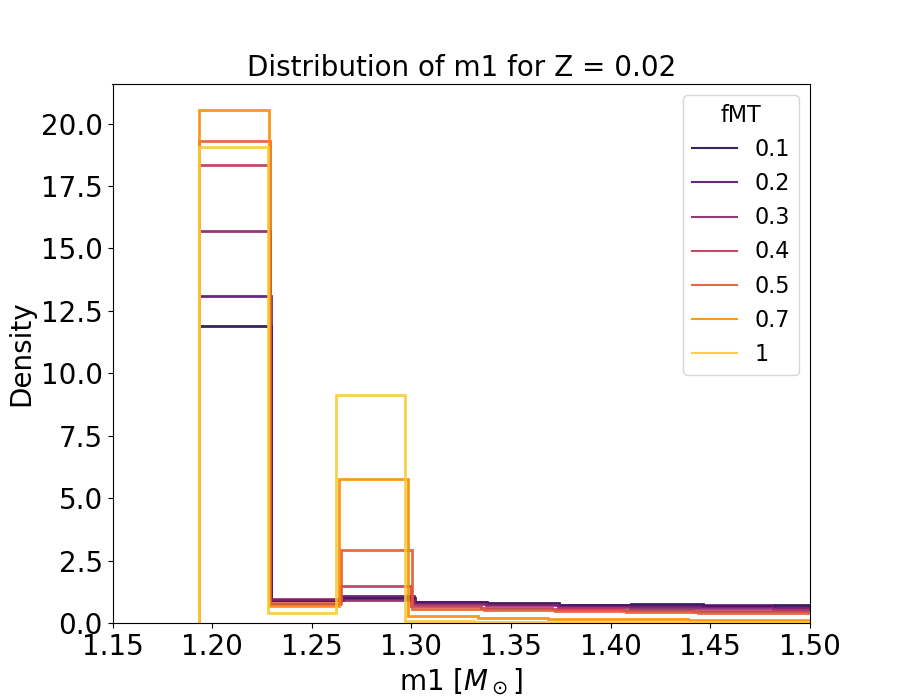
\includegraphics[width=1\textwidth]{Images/m1_zoom.png}
    \end{subfigure}
    \begin{subfigure}[t]{0.45\textwidth}
    \centering
        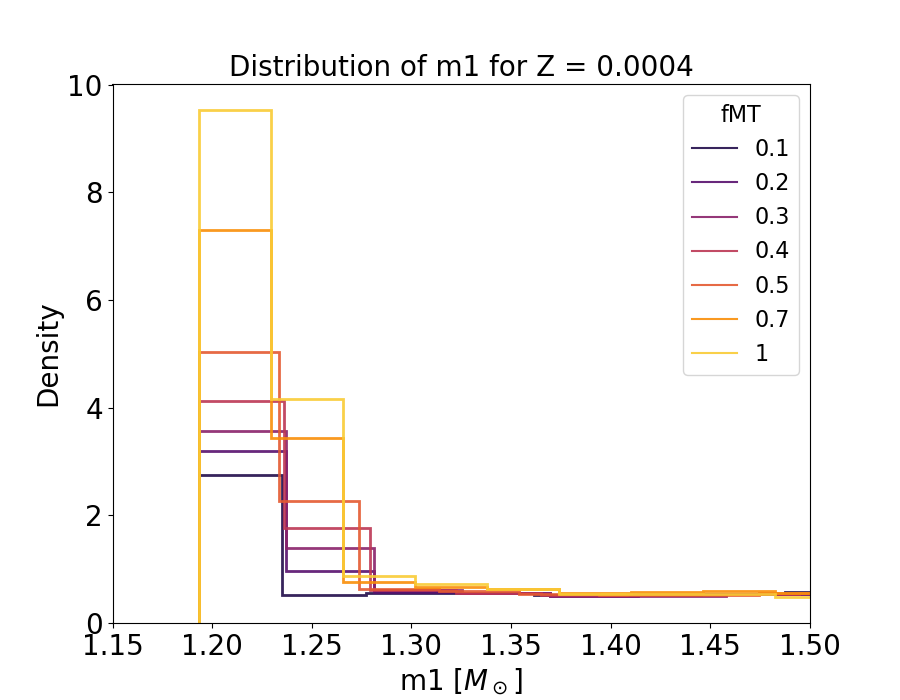
\includegraphics[width=1\textwidth]{Images/m1_zoomZ0.0004.png}
    \end{subfigure}
    \caption{Distribution of the first CO's mass.}
    \label{img:m1_zoom}
\end{figure}
    
\begin{figure}[ht]
    \centering
    \begin{subfigure}[t]{0.45\textwidth}
        \centering
        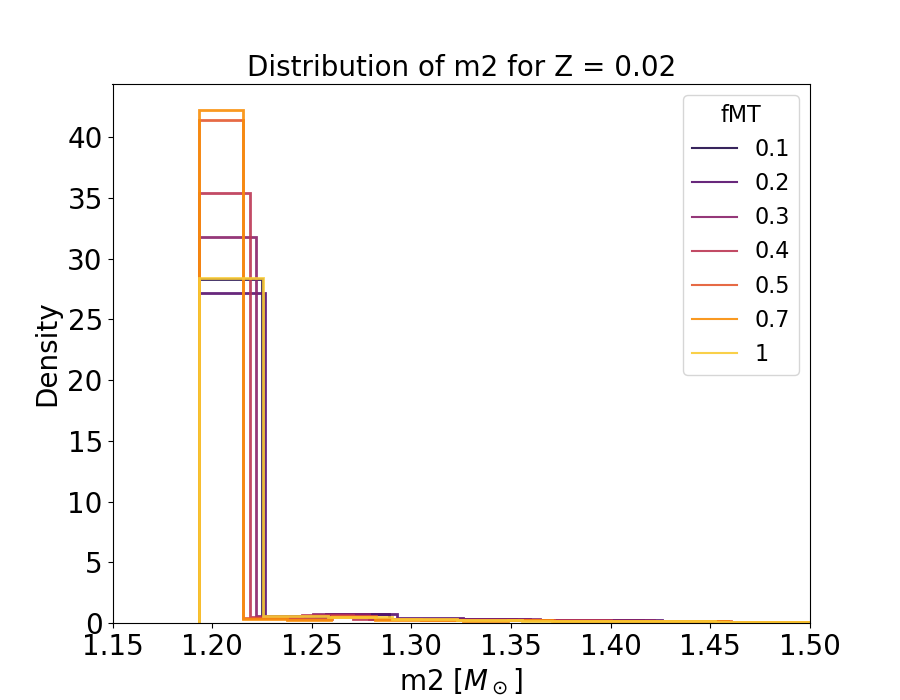
\includegraphics[width=1\textwidth]{Images/m2_zoom.png}   
    \end{subfigure}
    \begin{subfigure}[t]{0.45\textwidth}
    \centering 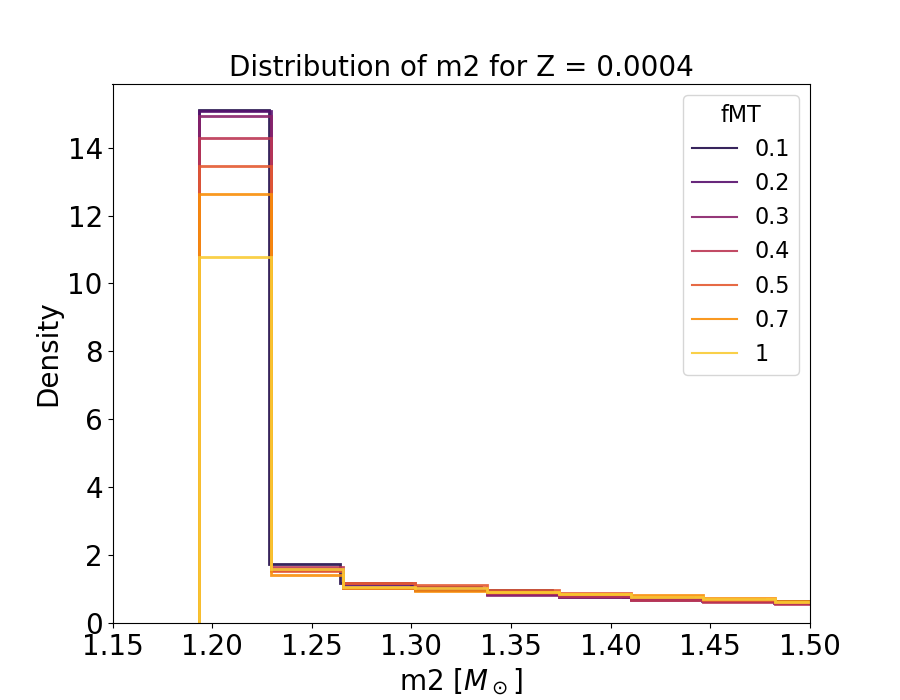
\includegraphics[width=1\textwidth]{Images/m2_zoomZ0.0004.png}
    \end{subfigure}
    \caption{Distribution of the second CO's mass.}
    \label{img:m2_zoom}
\end{figure}

Moreover, the distribution of the mass ratio ($q$) between the secondary and the primary CO is shown in the Fig.\ref{img:q}, this time for fixed $fMT$ and varying $Z$.
For $fMT=1$, the value of $q$ peaks around 1, and the number of counts is directly proportional to metallicity.  Interestingly, this behavior is also true for the smaller $fMT$.

\begin{figure}[h]
    \centering
    \begin{subfigure}[t]{0.45\textwidth}
        \centering
        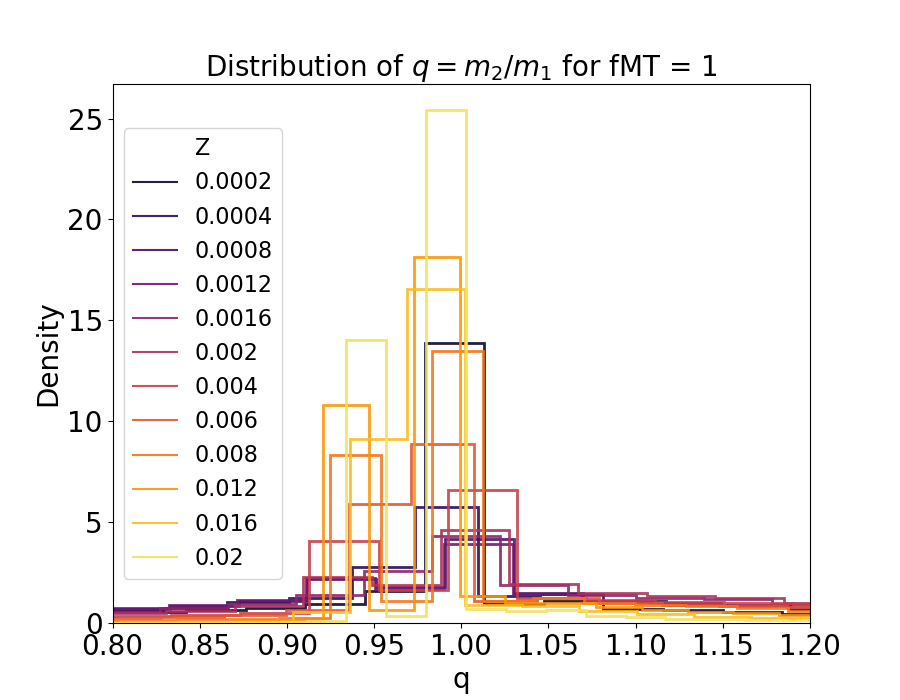
\includegraphics[width=1\textwidth]{Images/qfMT1.png}
    \end{subfigure}
    \begin{subfigure}[t]{0.45\textwidth}
        \centering    
        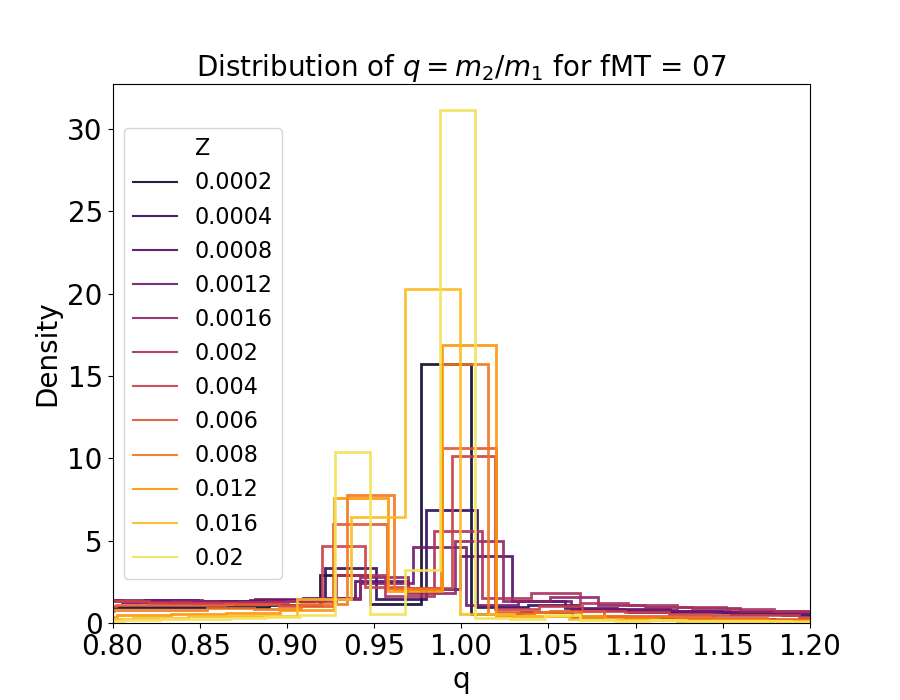
\includegraphics[width=1\textwidth]{Images/qfMT07.png}
    \end{subfigure}
\caption{Distribution of the mass ratio for $fMT=1$ and $fMT=0.7$.}
\label{img:q}
\end{figure}
\newpage

Fig.\ref{img:diff1} shows the distribution of the mass differences between $m_1$ and $m_2$, and the respective ZAMS masses. We notice that for higher values of fMT, the mass difference is smaller. This behavior is typical for different metallicities. From this plot, we restate that it is possible to have NS from more massive progenitors than expected. On the other hand, for an isolated star to form NS from a progenitor more massive than about $20M_{\odot}$ is not feasible. Also, the comparison between $Z=0.02$ and $Z=0.0004$, we notice that as $Z$ increases, the minimum mass to form a NS tends to shift more to the right. 

\\
\begin{figure}[ht]  
    \centering
    \begin{subfigure}[t]{0.45\textwidth}
        \centering
        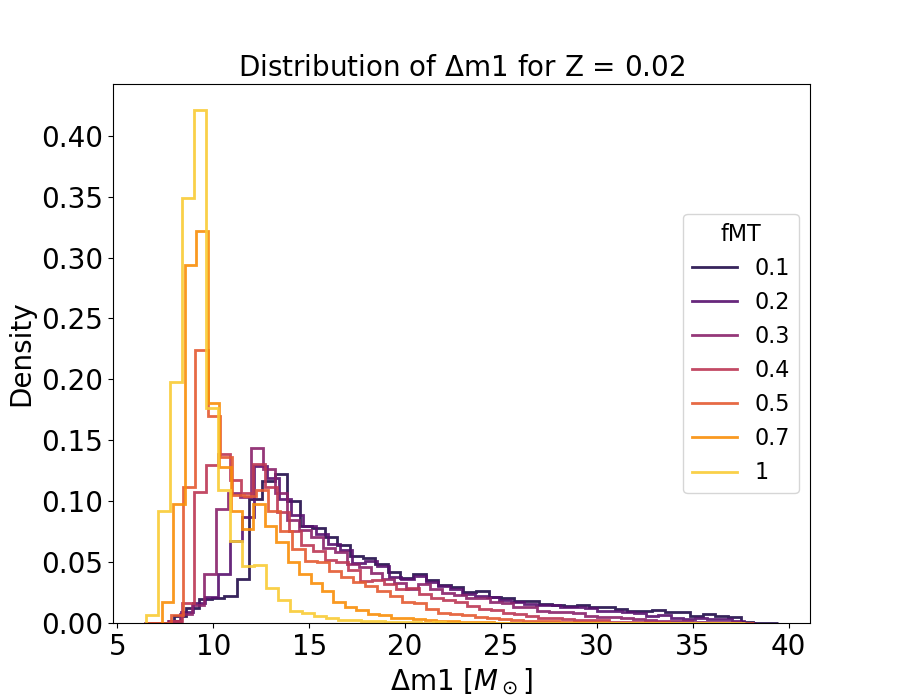
\includegraphics[width=1\textwidth]{Images/diff1.png}
    \end{subfigure}
    \begin{subfigure}[t]{0.45\textwidth}
        \centering  
        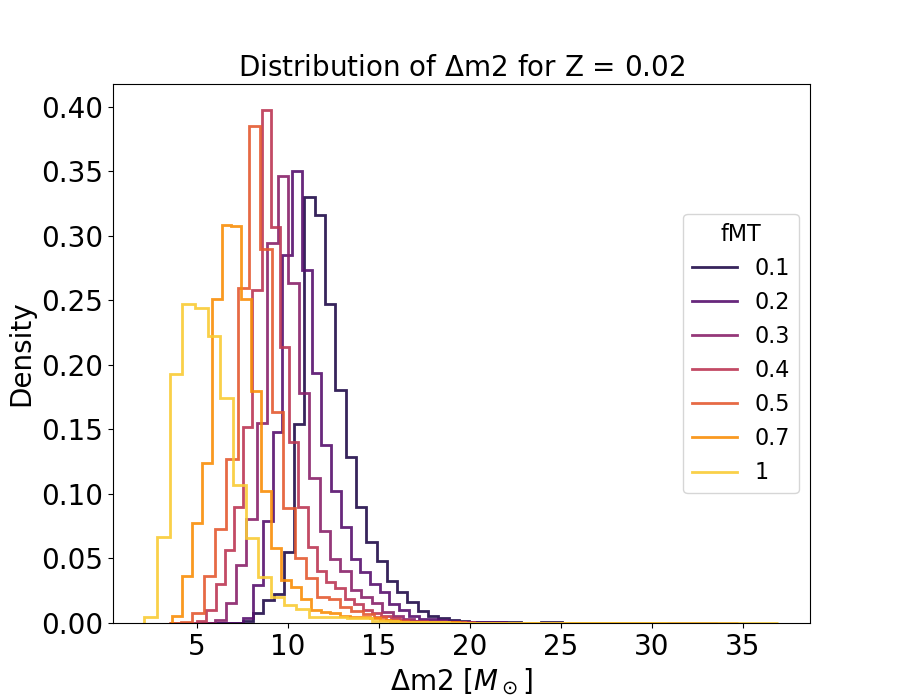
\includegraphics[width=1\textwidth]{Images/diff2.png}
    \end{subfigure}
    \begin{subfigure}[t]{0.45\textwidth}
        \centering  
        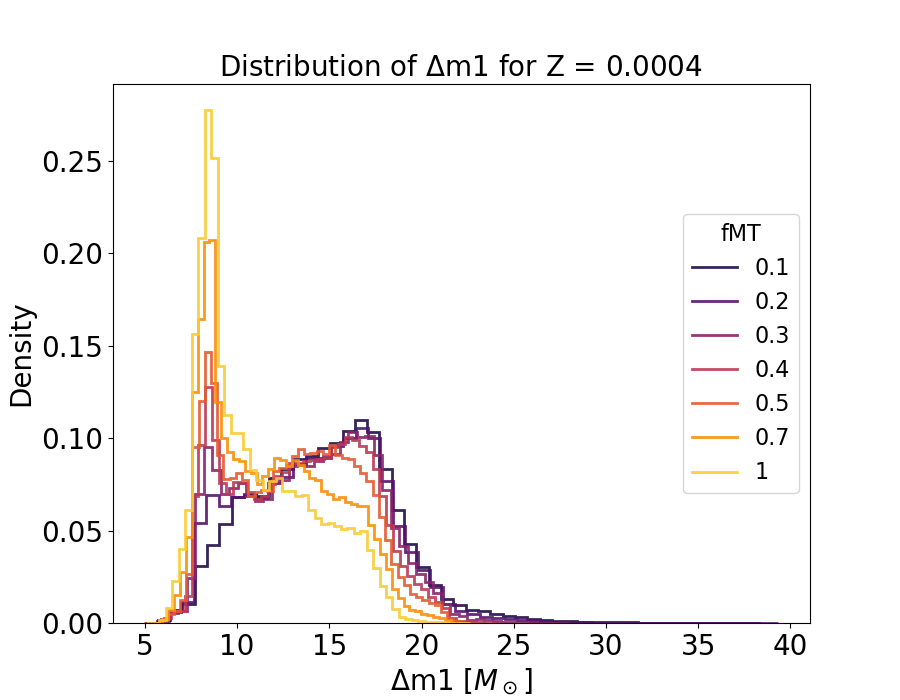
\includegraphics[width=1\textwidth]{Images/diff1Z0.0004.png}
    \end{subfigure}
    \begin{subfigure}[t]{0.45\textwidth}
        \centering  
        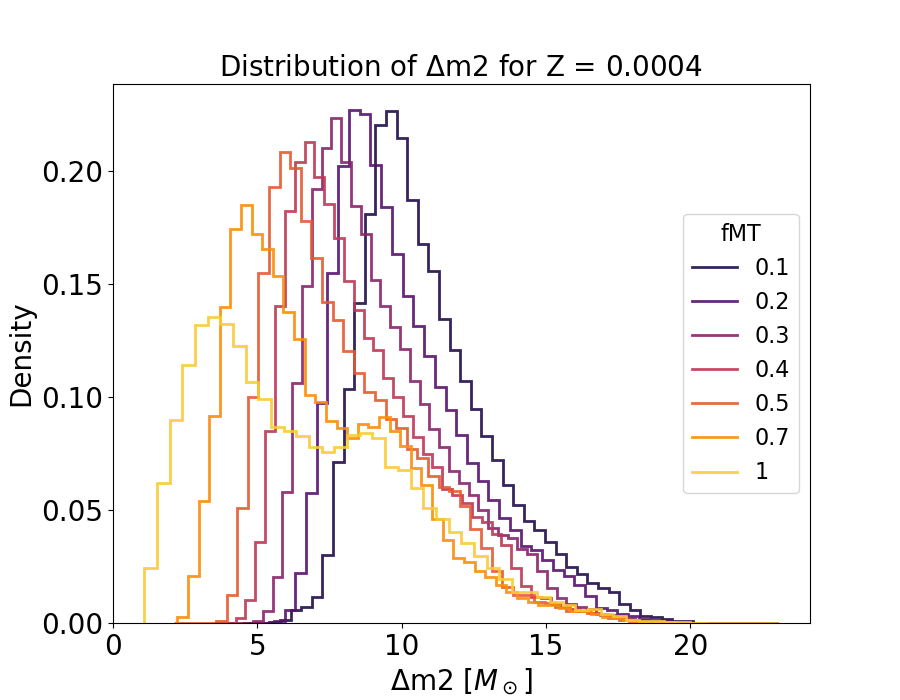
\includegraphics[width=1\textwidth]{Images/diff2Z0.0004.png}
    \end{subfigure}
    \caption{Distribution of the mass difference between the first and second CO and their progenitor star, for $Z=0.02$ and $Z=0.0004$.}
    \label{img:diff1}
 \end{figure}
 \\
 
To verify if the mass of the NS originating from the most massive progenitor is effectively larger than the mass of the other NS, the fraction of flipped masses between the primary and the secondary is plotted in Fig.\ref{img:flipmasses}, as a  function of $fMT$. From this plot, it is clear that for more efficient mass transfer, the fraction of flipped mass increases.
\begin{figure}[h!!]
    \centering
    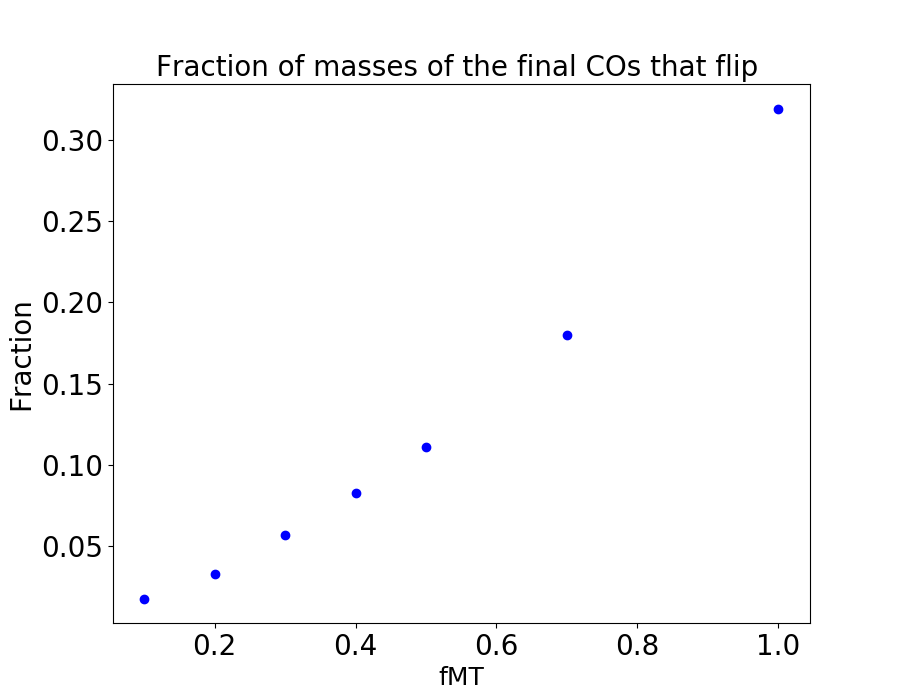
\includegraphics[width=0.6\textwidth]{Images/flipmasses.png}
    \caption{Plot of the fraction of the systems that presents flipped masses of the final COs with respect to the progenitors.}
    \label{img:flipmasses}
\end{figure}

\subsubsection{\textbf{Delay times - power law coefficient}}
The definition of Delay time in gravitational wave astronomy is the time between the stars formation and the coalescence of the binary compact objects.\\
To avoid the need to run the entire simulation for obtaining a set of delay times, we would want to estimate a global parameter that certainly should help us in describing the BNS population. By this way, we would be able to meaningfully sample from the selected population, and consequently analyze delay times.\\  
As we can see from the density graph in the log-log scale (Fig.\ref{img:delaytimes}), the density of delay times follows a linear behavior. We would like to determine the coefficient for all the systems, and its dependence on $fMT$, and $Z$, by using the time bounds from $10^2$-$10^4 Myr$. This procedure is quite handy to take into account only the linear part, thus neglecting the tails. Since we are considering the log-log scale, the original framework density of time delays obeys a power law of the kind:

\begin{align*}
    y(x) = b \cdot x^a
\end{align*}

The coefficient $a$ needs to be estimated, which is the slope returned by the linear regression.\\
Results of the fit depicted in Fig.\ref{img:a_vs_Z} and the values are computed by the mean of the method `polyfit' in the Python library `NumPy', that returns the regression line coefficients and errors given by the least-squares algorithm. 

\begin{figure}[htp]
    \begin{subfigure}[t]{0.50\textwidth}
      \centering
      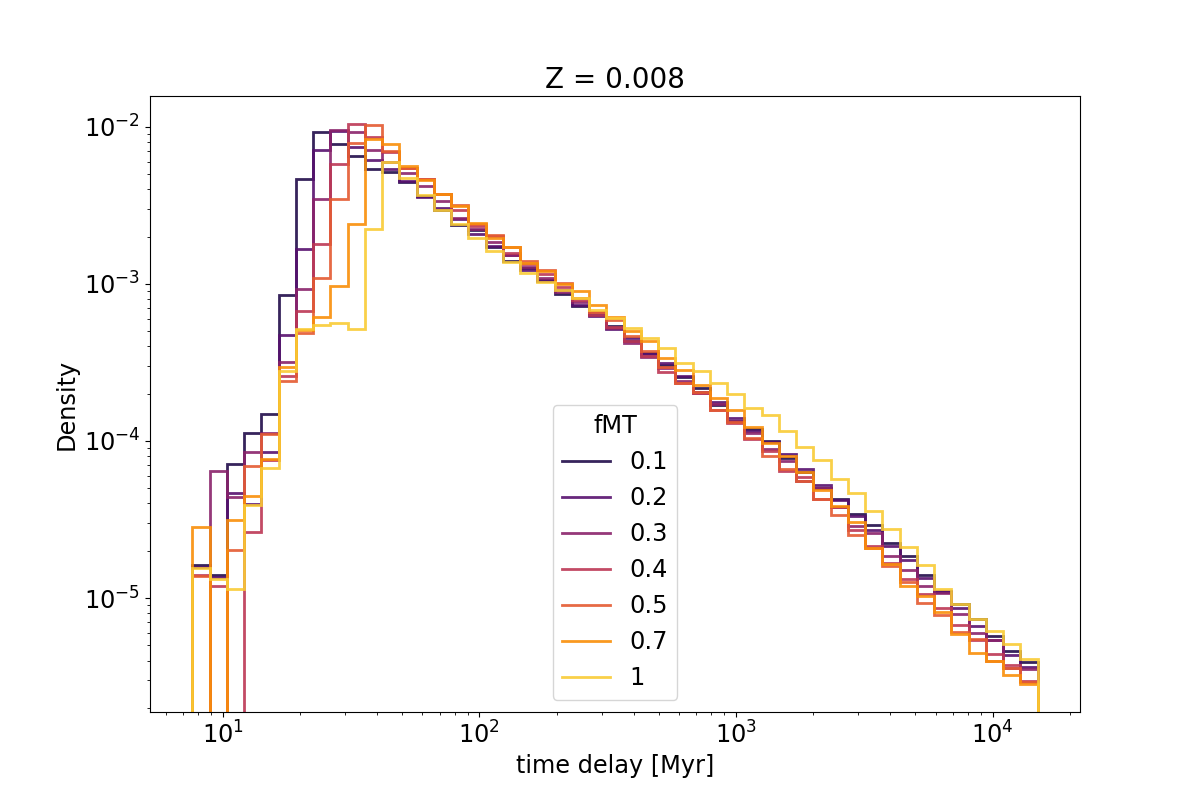
\includegraphics[width=1\textwidth]{Images/delaytimes_Z0.008.png}
      \caption{Distribution of delay times in log scale: since density is linear, a linear fit is used and the coefficients computed.}
      \label{img:delaytimes}
    \end{subfigure}
    \hfill
    \begin{subfigure}[t]{0.50\textwidth}
      \centering
      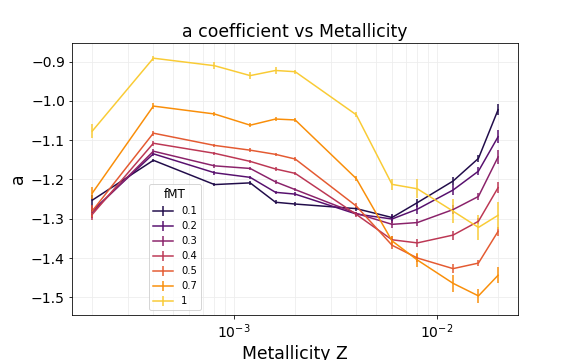
\includegraphics[width=1\textwidth]{Images/a_vs_Z.png}
      \caption{Coefficient `a' found for the slope of the density histograms as the function of the metallicity. Errors are found by the mean of the linear regression algorithm.}
      \label{img:a_vs_Z}
    \end{subfigure}
    \caption{Basic analysis for the `a' coefficient.}
    \label{img:a_coefficient_first}
  \end{figure}

These results show the exponent to be dependent on $Z$. Higher the mass transfer efficiency, the more probable is the delay times to be high at exponent being least, and the tail distribution becoming more relevant. Generally, this is valid up to $Z \sim 0.006$, where this behavior reverses: the curve indeed changes concavity, and we can consider at that particular metallicity as an inflection point.\\
However, it is worth pointing, as the $a$ coefficient clusters around at a certain value, we can, therefore, estimate its weighted mean taking into account of all the values that are obtained so far:

\begin{align}
   a = -1.24 \pm 0.13 \quad Myr^{-1}
   \label{value:a_coefficient}
\end{align}


\subsubsection{\textbf{Common Envelope phase}}
Another important subject is whether the system taken into account experiences a Common Envelope (CE) phase (briefed in the introductory section). When we analyze and look into the considered data, every system is associated with a label denoting the phase of evolution. The label `COMENV' refers to a CE phase just ended, which may be physically True or not. Thus we consider only the former, i.e., the ones that do not appear in the same line of the database of a previously formed BNS system. Whereas, the hypothetical ones refer to as ``cheat" of the simulation code, and are not to take into account.\\
In our work, we have primarily considered if a CE phase exists or not. Thanks to the following result Fig.\ref{img:count_CE_fraction}, one can see that the fraction of the system that does not go through the CE phase is statistically irrelevant. This is the raison d'être for our analysis, employing grouping binary systems based on the number of CE it goes through, assuming that one is the least. The existence of CE is a highly characteristic feature of BNS systems. It is highly unlikely to find the formation of BNS systems without a single CE phase in nature. 


\subsection{\textbf{Common Envelope - numbers}}

Speaking in terms of statistics, the systems that do not undergo the CE phase are judged irrelevant in our analysis. Generally, there is a possibility of the CE phase occurring more than once for a single system. The number of CE phases can reach up to three in number. We split our events according to this count, and finally, normalize it to total systems. Curves describing these fraction as a function of $Z$ and efficiency of mass transfer is shown in the Fig.\ref{img:count_CE_fraction}. 

\begin{figure}[ht]
    \begin{subfigure}[t]{1\textwidth}
      \centering
       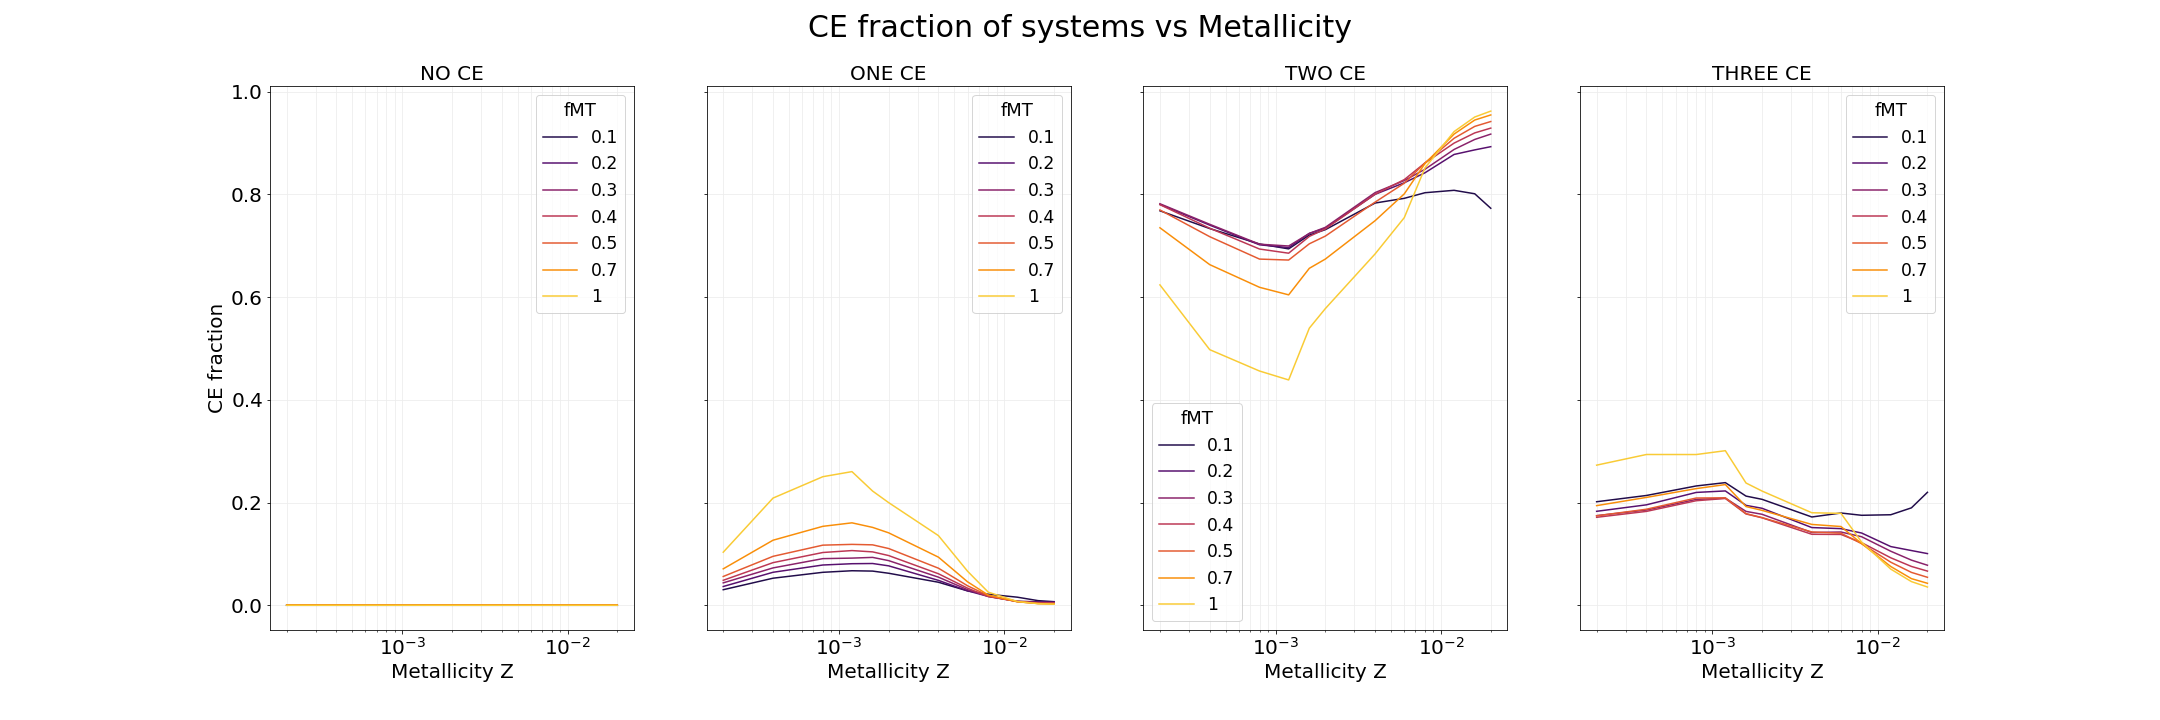
\includegraphics[width=1\textwidth]{Images/count_CE_vs_metallicity.png}
       \caption{}
       \label{img:count_CE_vs_Z}
    \end{subfigure}
    \begin{subfigure}[t]{1\textwidth}
      \centering
      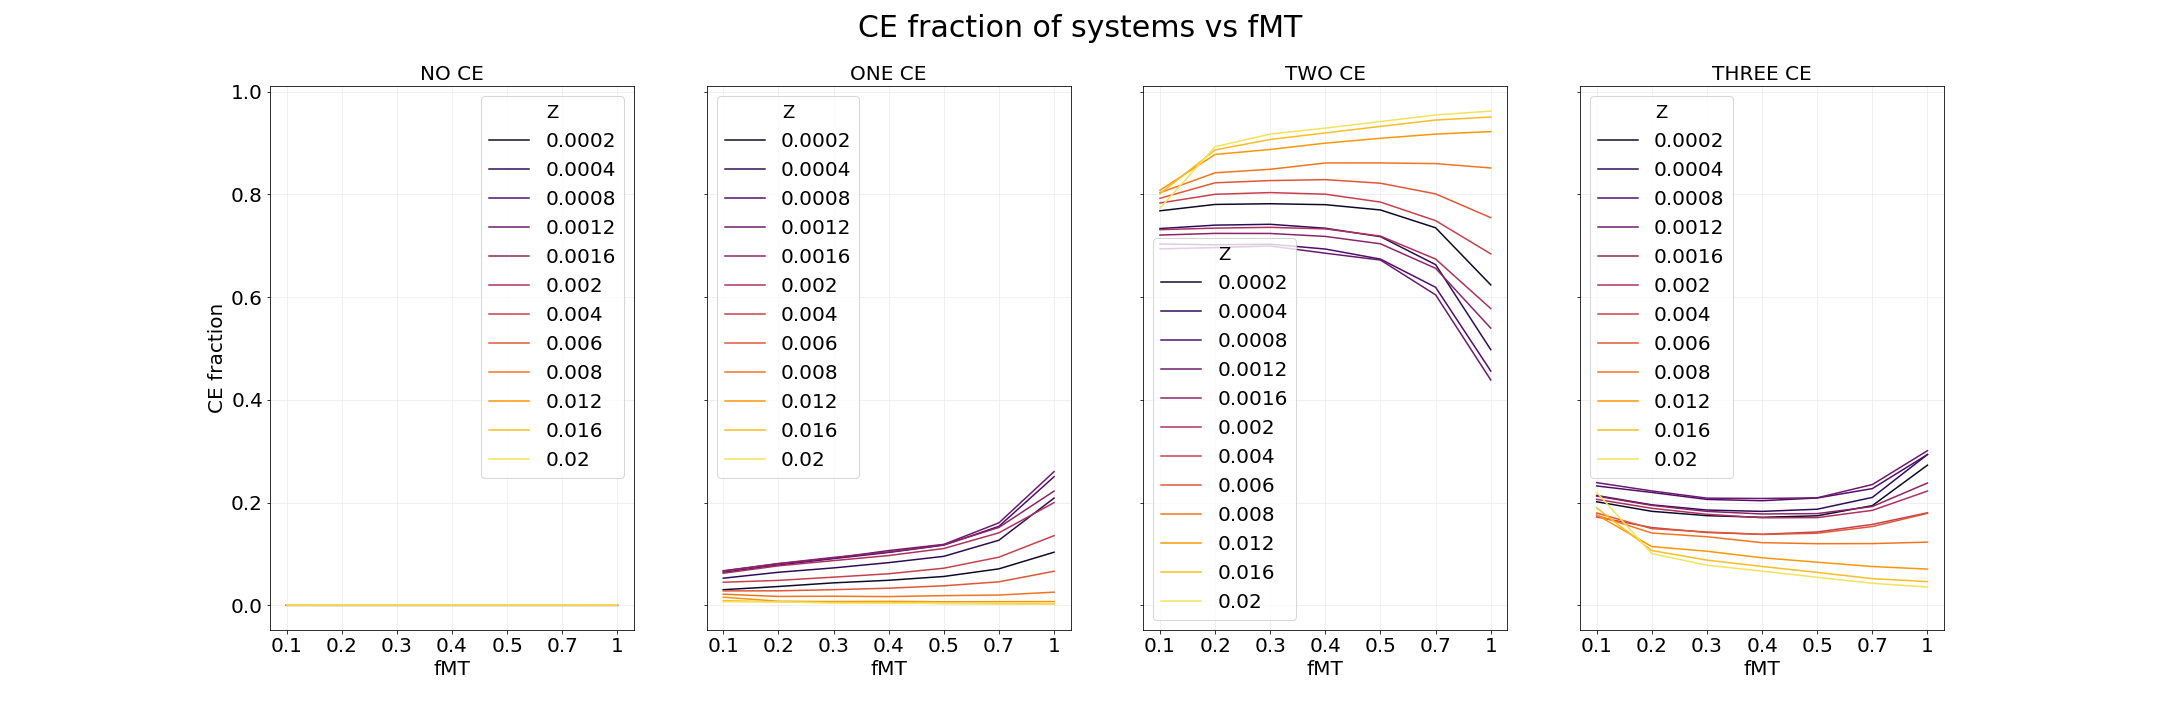
\includegraphics[width=1\textwidth]{Images/count_CE_vs_fMT.png}
      \label{img:CE_count_vs_fMT}
      \caption{}
    \end{subfigure} 
    \caption{Fraction of systems and corresponding number of CE for different $Z$ and $fMT$.}
    \label{img:count_CE_fraction}
\end{figure}

One can easily notice that almost every system experiences at least one CE phase during its lifetime. More likely to face two CEs. There is an important feature to note: the increase in $Z$ leads to the increase of the CE fraction, as shown in Fig.\ref{img:count_CE_fraction}, i.e., favoring two CE phases formation. For one CE and three CE phase is the contrary effect (low $Z$). Another interesting feature for all the curves in Fig.\ref{img:a_vs_fMT_CE_count}, there exists a stationary point around $ Z \sim 0.001$.\\

\subsubsection{\textbf{Types of CE}}
\label{sec:type_CE}

We label our CE phase according to all possible cases in which it might occur. The combination is represented as:
\begin{itemize}
    \item \textbf{1A} $\quad \text{star}$ + $\text{star} \rightarrow  \text{star'}$ + $\text{star'}$
    \item \textbf{1B} $\quad \text{star}$ + $\text{star} \rightarrow  \text{NS}$ + $\text{star'}$
    \item \textbf{1C} $\quad \text{star}$ + $\text{star} \rightarrow  \text{NS}$ + $\text{NS}$
    \item \textbf{2A} $\quad \text{NS}$ + $\text{star} \rightarrow  \text{NS}$ + $\text{star'}$
    \item \textbf{2B} $\quad \text{NS}$ + $\text{star} \rightarrow  \text{NS}$ + $\text{NS}$
\end{itemize}
\\

Where \textit{star} is referred to a star that is yet to become a NS.\\

It is interesting to analyze a few special cases for systems where only a single, as well as two or three, CEs occur. Here all the possible combinations for the CE to occur given by their number for a certain system are produced.

\begin{figure}[htp]
    \begin{subfigure}[t]{1\textwidth}
    \centering
        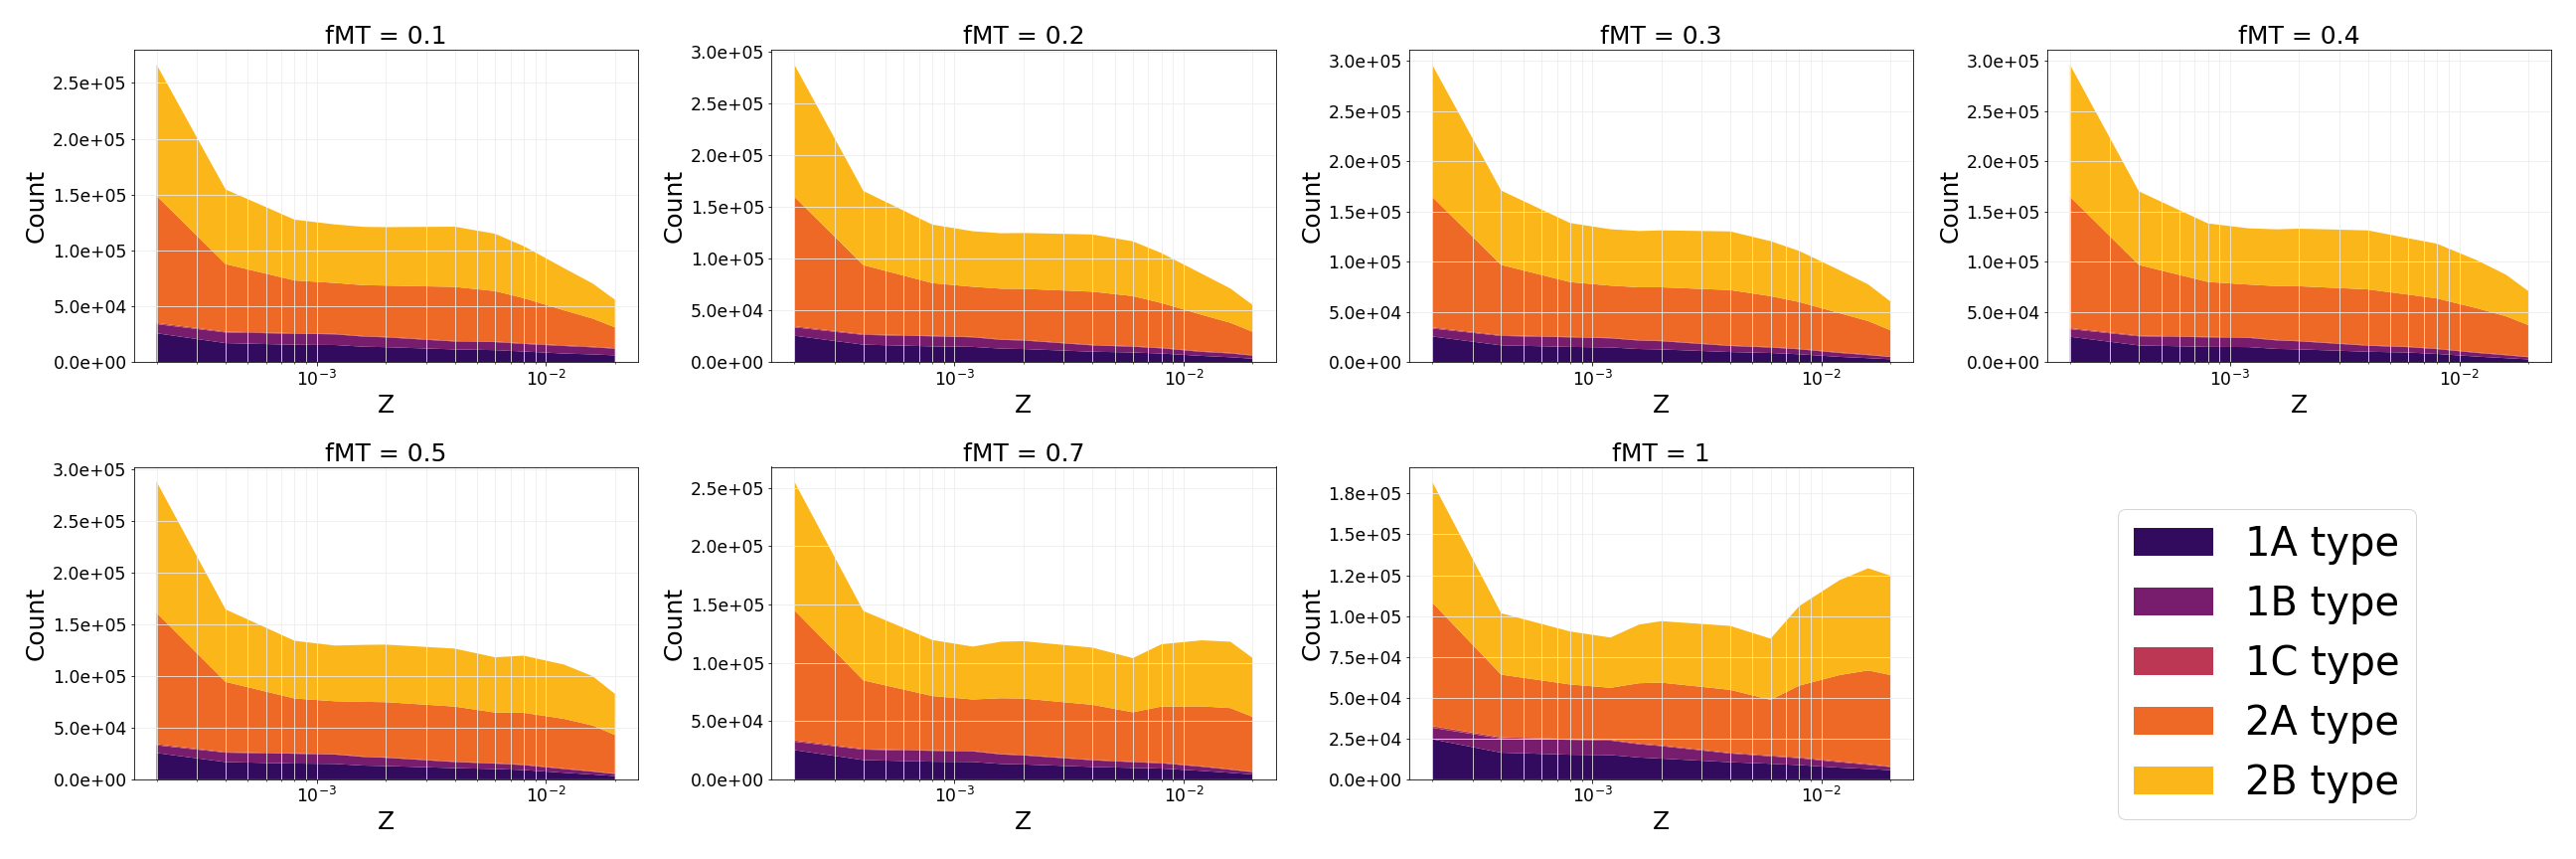
\includegraphics[width=1\textwidth]{Images/ONE_CE_which.png}
        \caption{Count of CE grouped per type, given only ONE has occurred.}
        \label{img:ONE_CE_which}
    \end{subfigure}
    \hfill
    \begin{subfigure}[t]{1\textwidth}
        \centering
        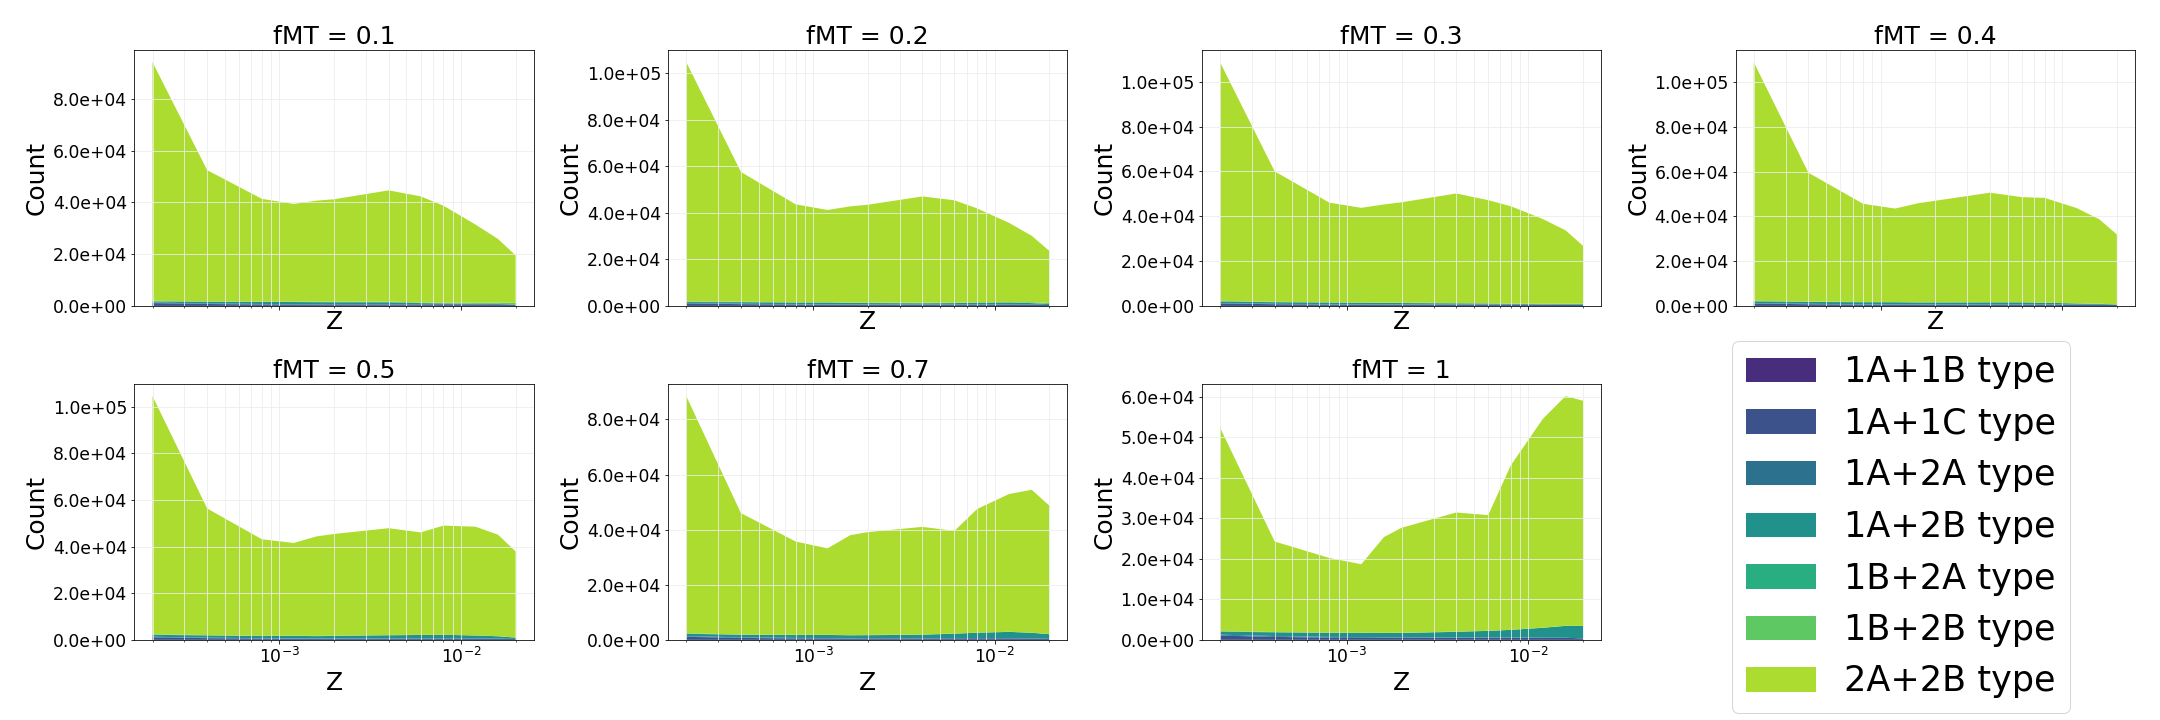
\includegraphics[width=1\textwidth]{Images/TWO_CE_which.png}
        \caption{Count of CE grouped per type, given TWO have occurred.}
        \label{img:TWO_CE_which}
    \end{subfigure} 
    \hfill
    \begin{subfigure}[t]{1\textwidth}
      \centering
      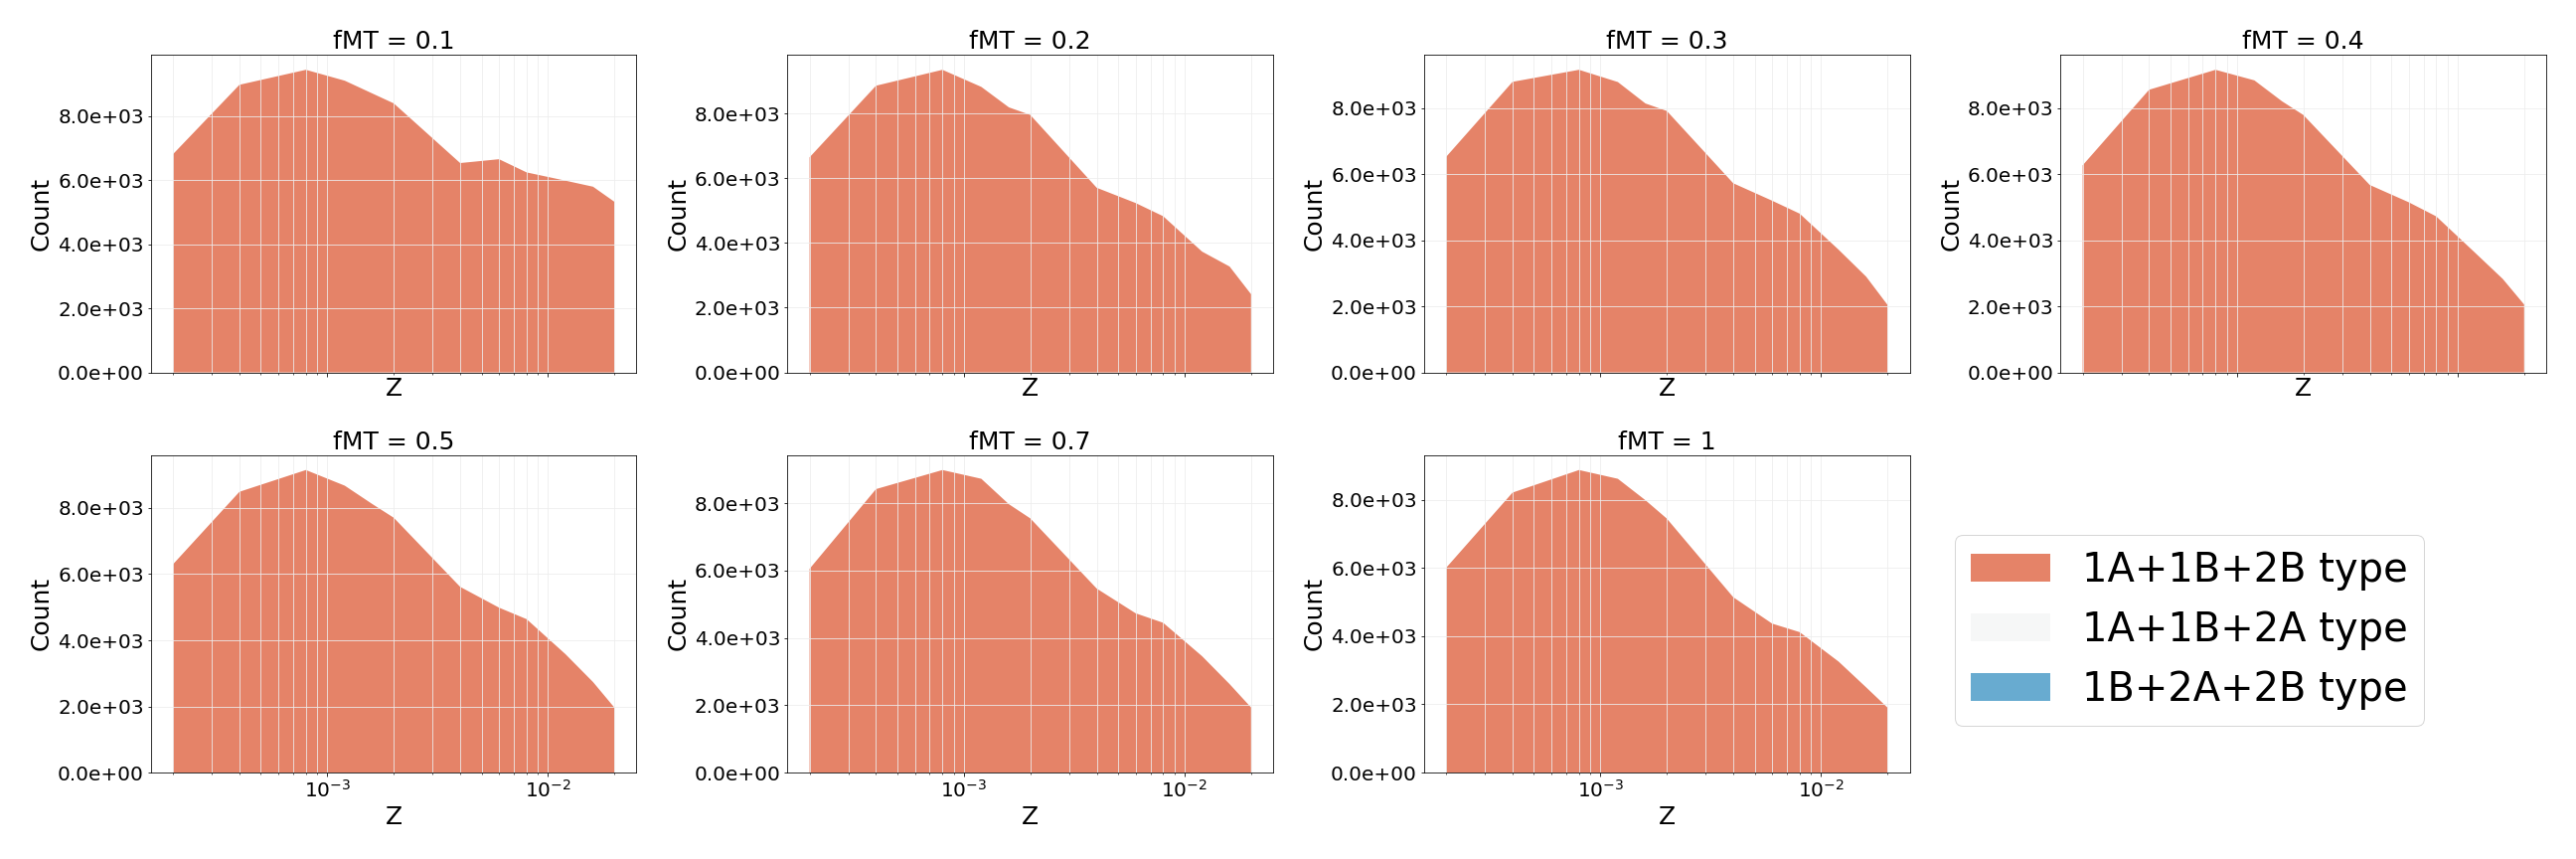
\includegraphics[width=1\textwidth]{Images/THREE_CE_which.png}
      \caption{Count of CE grouped per type, given THREE have occurred.}
      \label{img:THREE_CE_which}
    \end{subfigure} 
    \caption{Plots depicting the different number of CEs, type, or combination of types, is more likely to occur. Scale is chosen not to be log-log one in order to visualize data in a better and clearer way: The larger is the area related to a single color, the more a specific type of CE is observed.}
    \label{img:number_CE_which}
\end{figure}

The Fig.\ref{img:ONE_CE_which} gives us information about the types of CEs formed. The systems with one CE is said to have a higher probability for one of the binary to be a NS (already formed). Moreover, the higher the metallicity, the lesser number of systems with two stars experience a CE ($1A, 1B, 1C$ type, darker colors in the plots). Additionally, the largest number of CEs is related to low metallicities for all $fMT$s. Also, we notice a change in behavior after the point of $Z \sim 0.006$. For low $fMT$s, CE events decrease, whereas, for high values, it increases. It might be because of ineffective mass transfer by not filling the Roche lobes, CE fails to occur or is comparatively quite low. Finally, we infer that there are almost no statistics for $\mathbf{1C}$ type. Therefore it is highly unlikely for two stars to experience a CE, and both of them turning out to be BNS. Despite the lack of statistics, it is still an interesting topic for future works. Since these kinds of systems exist, one would like to investigate them.\\

An initial remark about Fig.\ref{img:TWO_CE_which} is by considering systems with two CE, we are indeed taking into the majority of systems for our database. This is concluded by the courtesy of Fig.\ref{img:count_CE_fraction}. One may note that almost all the statistics is covered by the combination of types referring to CE occurring with a NS already formed. One of the possible interpretations for the case where the system goes through two CE is the following, especially if the times between them is relatively short: once the primary progenitor is already a NS, the secondary may go through the first CE, therefore, ejecting its hydrogen envelope if the spiraling has sufficient energy to do so. At this moment, simulation takes into account the change of phase for the second object, and we are left with a binary system where the first object is already a NS, and the second one is a Wolf-Rayet star (WR). From now on, the latter starts evolving as a naked helium core. After a short time compared to the star's lifespan, but sufficiently large compared to a WR average lifetime, there exists a non-null probability that the helium layer of the secondary object is ejected as well, thanks to a Common Envelope. The plot (Fig.\ref{img:diff_time_2A_2B}) endorses our hypothesis and tells us that there might be such events, being present also the aforementioned short times in the histogram.
%lecture_2020_05_22_WASConly, h1 min02

\begin{figure}[h!]
    \centering
    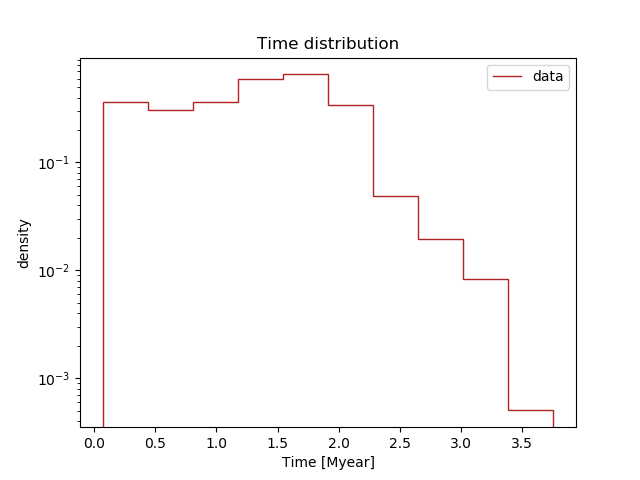
\includegraphics[width=0.5\textwidth]{Images/2A_2B_time_difference.png}
    \caption{Histogram for times spent between two consecutive 2A and 2B CEs. Here are taken into account all systems that undergo these two CEs.}
    \label{img:diff_time_2A_2B}
\end{figure}
\\

According to Fig.\ref{img:TWO_CE_which}, we observe a strong change in behavior after $Z \sim 0.006$, depending on $fMT$. For low $fMT$ total number of events counted decreases, instead of $fMT \geqslant 0.5$, it first flattens and then increases. For metallicities lower than $Z \sim 0.006$ point, graphs do not show any higher variation. For high mass transfer efficiency, probability of CE between two stars that may change the type and finally not ending up as a NS is seen to slightly increase, but still being negligible concerning the other cases.\\
However, Fig.\ref{img:THREE_CE_which} shows out of the five possible CE combinations, the one where two stars change type after a CE phase is $1A$. Hence one of them becomes a NS ($1B$), and finally, the last CE leads its companion to become a NS itself ($2B$). For ($2A$, $2B$) the same reason is valid as stated before, therefore $2A$ and $2B$ may refer to two CEs one shortly after the other one (see Fig.\ref{img:diff_time_2A_2B}). For three events of CE, we observe that the behavior is unique for every $fMT$ parameter, except for $0.1$, where we count a larger number of events. This is indeed coherent with the result previously obtained in Fig.\ref{img:count_CE_fraction}a.\\ 

\subsubsection{\textbf{Power law coefficient}}

We grouped systems by the number of CE they undergo and plotted their delay times density histogram. Since their distribution is linear in the log-log scale, we apply a similar analysis to the one we have previously used to estimate the slope of the fitting line, namely the $a$ coefficient.

\begin{figure}[htp]
    \begin{subfigure}[t]{1\textwidth}
      \centering
      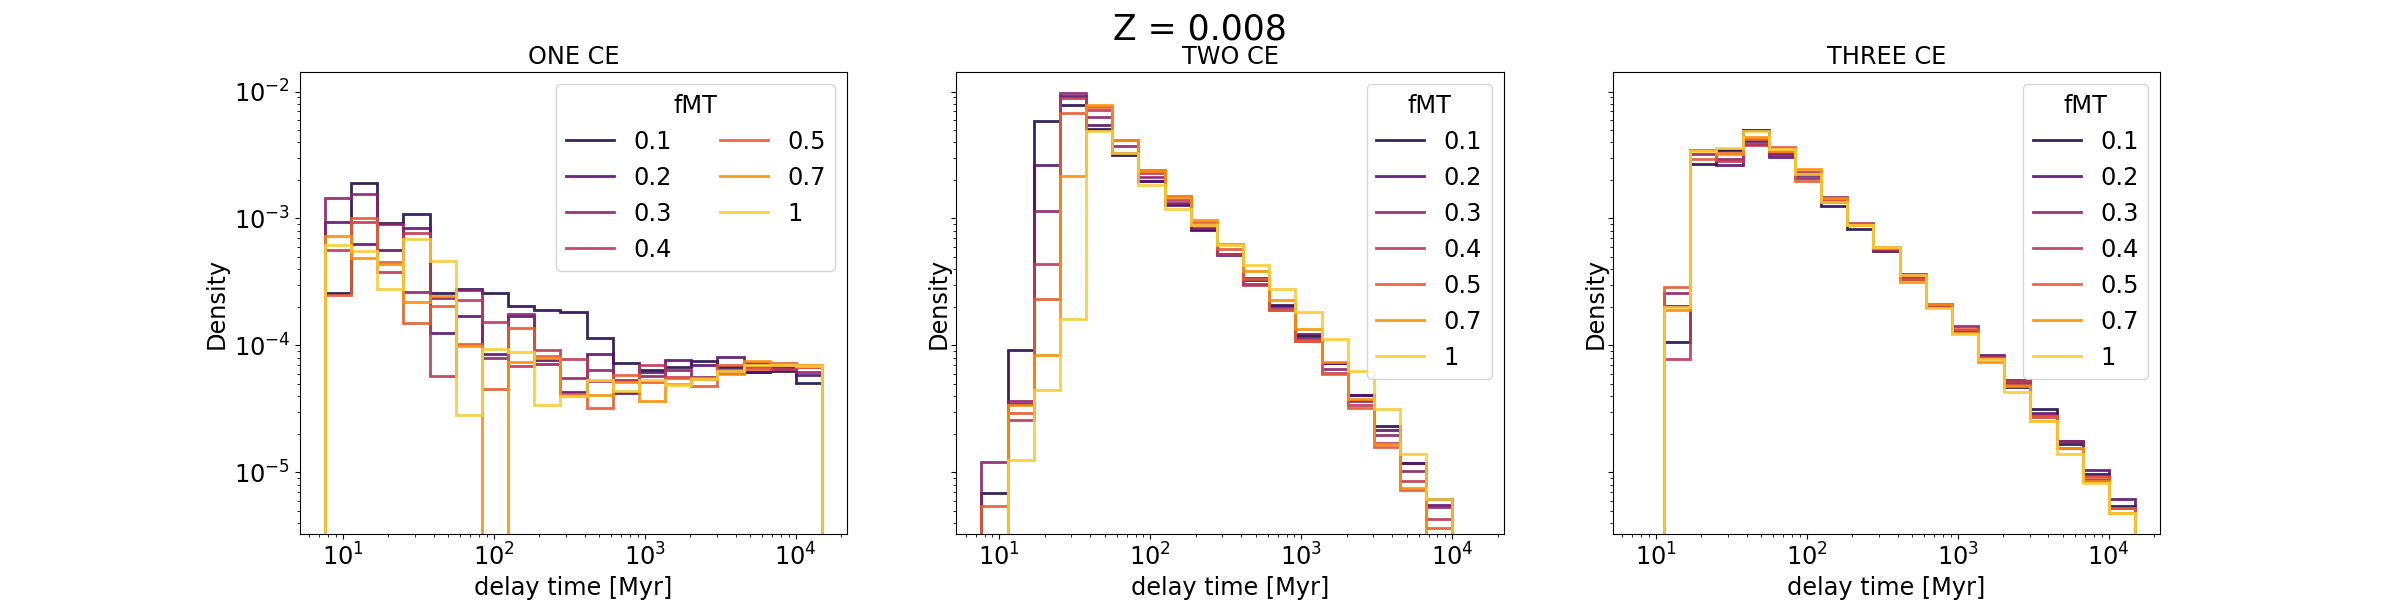
\includegraphics[width=1\textwidth]{Images/delaytimes_Z0.008_CEcount.png}
      \caption{Density of delay times in log-log scale for different numbers of CEs.}
      \label{img:delaytimes_count_CE}
    \end{subfigure}
    \begin{subfigure}[t]{1\textwidth}
      \centering
      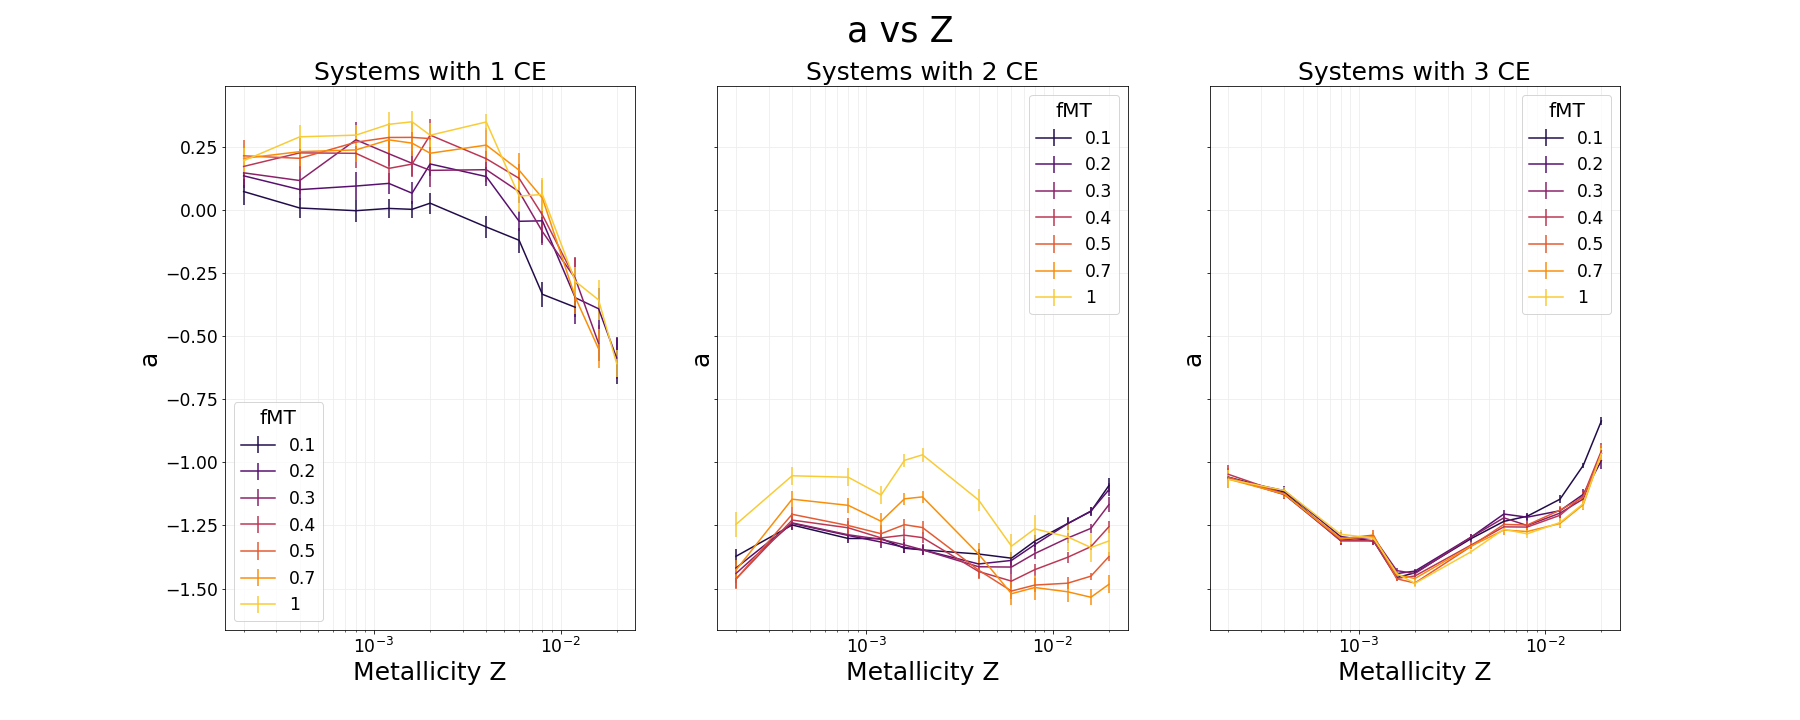
\includegraphics[width=1\textwidth]{Images/a_vs_Z_CE_count.png}
      \caption{Coefficient $a$ is found for the slope of the density histograms as the  function of $Z$. Errors are found by the mean of the linear regression algorithm.}
      \label{img:a_vs_Z_CE_count}
    \end{subfigure}
    \hfill
    \begin{subfigure}[t]{1\textwidth}
      \centering
      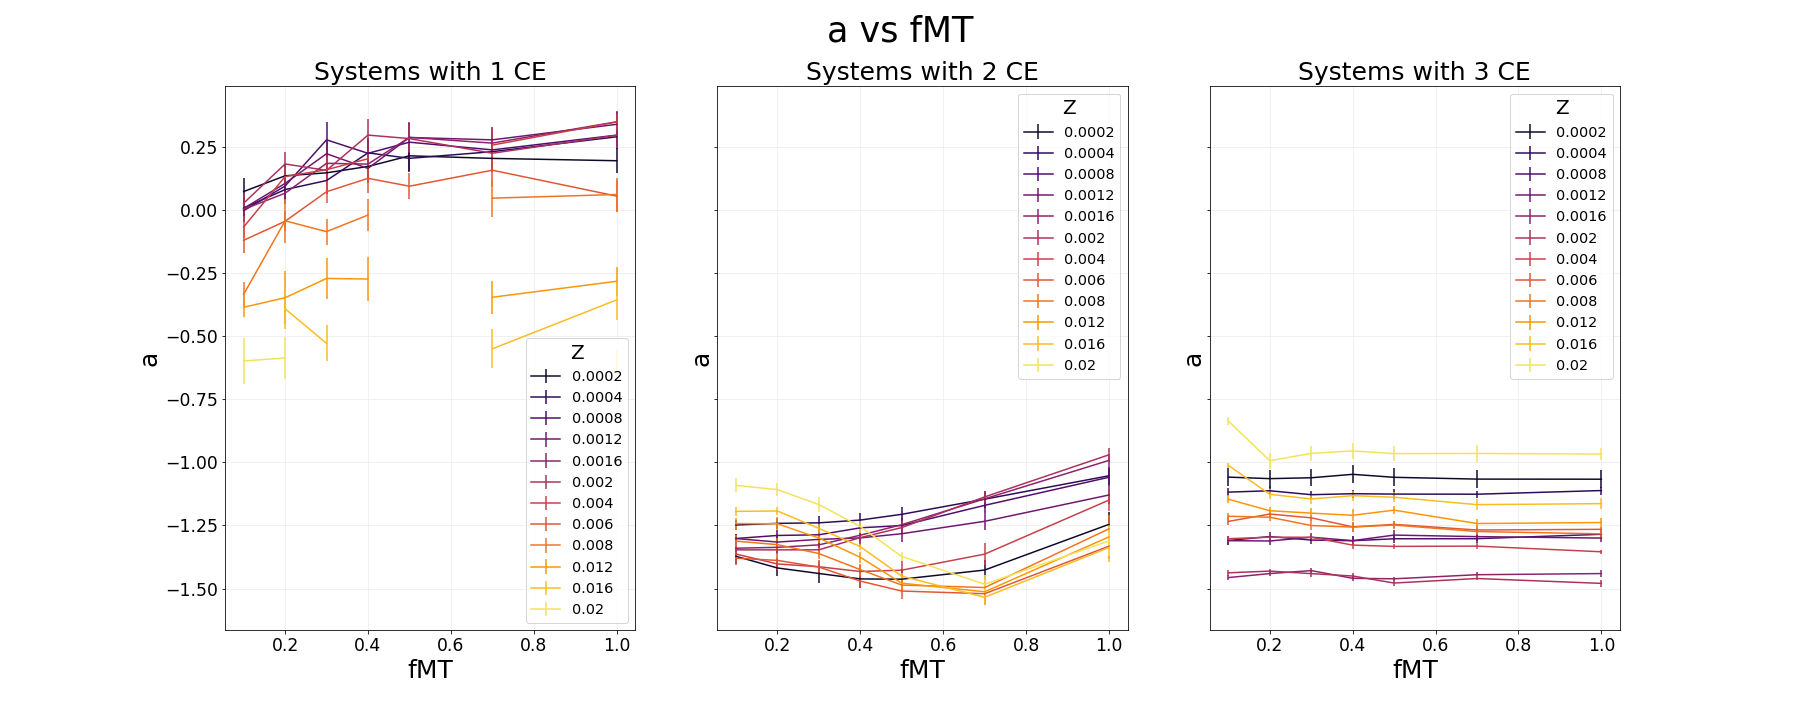
\includegraphics[width=1\textwidth]{Images/a_vs_fMT_CE_count.png}
      \caption{Coefficient $a$ is found for the slope of the density histograms in function of the $fMT$. Errors are found by the mean of the linear regression algorithm.}
      \label{img:a_vs_fMT_CE_count}
    \end{subfigure}
    \caption{Basic analysis for the $a$ coefficient.}
  \end{figure}

An interesting feature from Fig.\ref{img:delaytimes_count_CE} is that the systems with only one 'CE' can be fitted by a $flat$ line. Indeed the $a$ coefficient (Fig.\ref{img:a_vs_Z_CE_count}) for low metallicities is related to this subset of data, and is collocated around 0, which is the slope, and is expected from the plots. Other plots, present in the GitHub \citep{github}, describes this ``noisy" behavior for high $Z$. In the region around $Z \sim 0.006$, there is a notable change in behavior of the curve. On the other hand, for two and three CEs, curves are very similar and coherent one to each other. Once again, we stress the value of $Z \sim 0.006$ to be region-specific, where especially for the graph in the center, lines cross each other. Finally, three CE phases curve almost coincide.\\

From the previous plot (Fig.\ref{img:a_vs_fMT_CE_count}), we determine that for low metallicities, $a$ coefficient is independent of $fMT$. Whereas it is a sensible change to go higher with $Z$, and its values are different. The reason for this is explained by the mean of (Fig.\ref{img:count_CE_fraction}): For high $Z$, we see that very few systems do only one CE, so the statistic is low to estimate $a$ correctly. This comes in handy to tell us why there is a discontinuity for high $Z$, and a few values of $a$ are either missing or are sparser. Physically, it would mean that the system undergoes a single CE, then delay times will tend to be larger. Note that a discontinuity (i.e., a lack of value in the plot), is due to the non-convergence of the algorithm used to make the linear regression. Contributions by small metallicities may return a positive value for the $a$ coefficient, that in turn would make the distributions of delay time peak towards even higher times.\\
Putting the pieces together, we summarise our result into the following table \ref{table:a_coefficient} for systems with different numbers of CE:

\begin{table}[h!]
\centering
\begin{tabular}{||c c c c||} 
 \hline
   & \textbf{1 CE} & \textbf{2 CE} & \textbf{3 CE}  \\ [0.5ex] 
 \hline\hline
 $a$ coefficient \footnotesize{ $[Myr^{-1}]$ } &  0.01 $\pm$ 0.27 & -1.31 $\pm$ 0.13 & -1.19 $\pm$ 0.15\\
 \hline
\end{tabular}
\caption{Table depicting the value of the $a$ coefficient for the power law related to delay times density. Values are computed by using weighted mean and its error.}
\label{table:a_coefficient}
\end{table}

As already mentioned that delay times for one CE system are way longer, this might be due to the lack of statistics related to those systems, or eventually to the physics hiding behind this phenomenon is to be investigated thoroughly. The first hypothesis is more probable according to the uncertainty, which is almost doubled for one CE systems.

\subsubsection{\textbf{Mass density scatter-plots}}

Based on the number of CE's that a system might undergo, we obtain the scatter plot for the masses $m_1$ and $m_2$.\\
We choose as initial masses the ones in the database with label \textit{`INITIAL'} and are considered to be at time zero (clearly for systems that end up being BNS). Therefore, we consider the masses of their progenitors. The final mass is those of the compact objects.

\begin{figure}[ht]
    \begin{subfigure}[t]{1\textwidth}
      \centering
      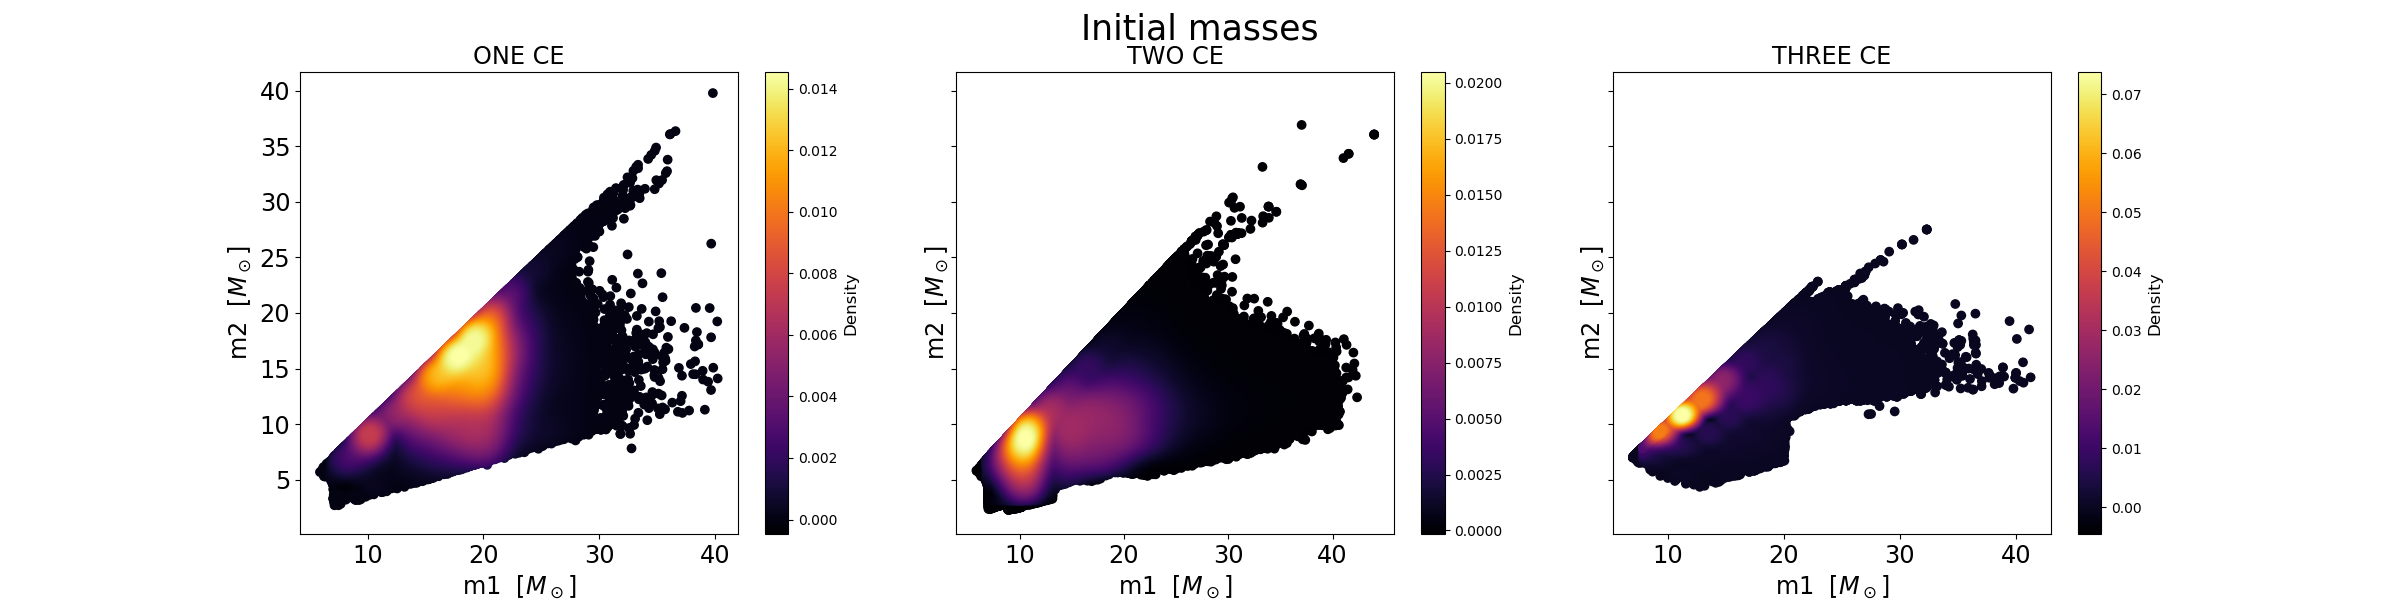
\includegraphics[width=1\textwidth]{Images/Initial masses_scatter.png}
      \caption{Scatter density plot:Initial mass 1 and mass 2 of the progenitors for all $fMT$ and all $Z$.}
    \label{img:scatter_initial}
    \end{subfigure}
    \begin{subfigure}[t]{1\textwidth}
      \centering
      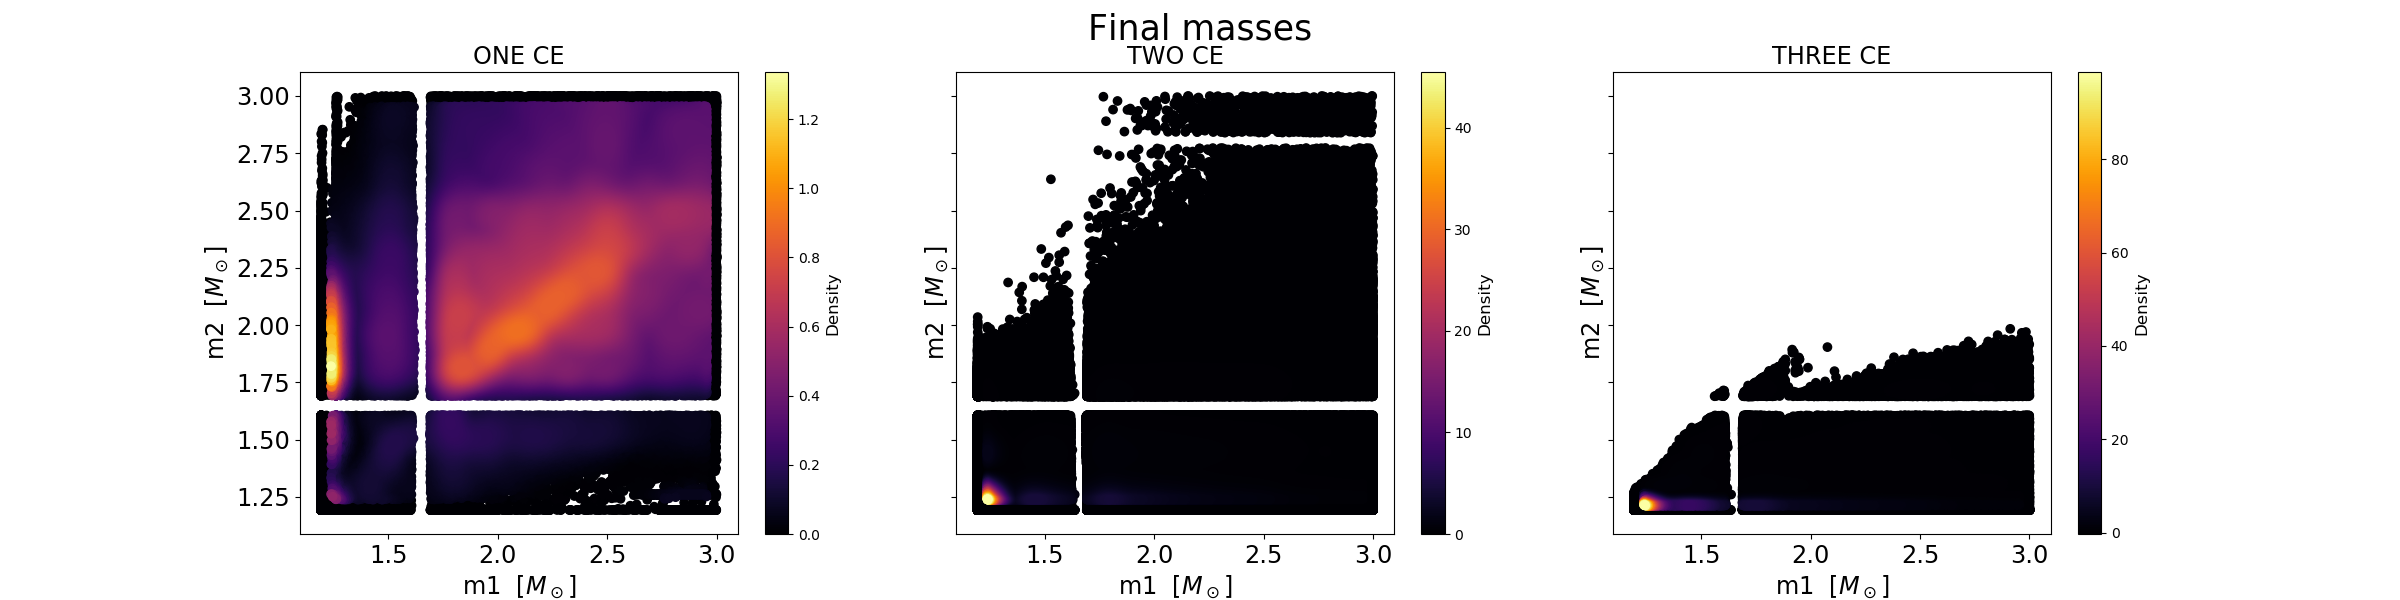
\includegraphics[width=1\textwidth]{Images/Final masses_scatter.png}
      \caption{Scatter density plot:Final mass 1 and mass 2 of the NS before merger for all $fMT$ and all $Z$.}
    \label{img:scatter_final}
    \end{subfigure}
    \caption{Scatter density plots of masses of progenitors and compact objects generated after them.}
    \label{img:scatter_plots}
 \end{figure}

According to the Fig.\ref{img:scatter_initial}, mass distribution of systems that experience one CE phase are highly concentrated between $15 M_\odot-20 M_\odot$. The BNSs formed are from the massive progenitors. The progenitors, in this case, are close to (or above) the maximum ZAMS mass to become a NS. This implies that consistent mass loss has happened, because of binary evolution. Moreover, these massive stars are much rarer than $\sim 8-12 M_{\odot}$ stars, because of the slope of the initial mass function. Distribution for one CE is relatively broader than the two and three CE. Generally, for higher masses, we tend to have only one CE, while for masses around $(10-12 M_\odot, 8-10 M_\odot)$ either two or three. These are relatively low masses, and according to Fig.\ref{img:count_CE_vs_Z} are the most statistically relevant systems in our population\citep{Kroupa:2001, Salpeter:1955}. For almost equal masses, namely for points lying on the bisector line, there is a possibility of the system undergoing three CE.\\

The Fig.(\ref{img:scatter_final}) suggests a discontinuity in the scatter plots. This is an effect of Fryer prescription \citep{Fryer:2012}. We recognize a general trend in the number of CEs a system goes through concerning its masses "flipped" (compact objects generated by the most massive progenitor become the least massive ones). If the systems undergo a higher number of CEs, then the probability of its masses flipped is low. Besides, increasing the number of CE, it can be seen that the majority of systems tend to lie below the bisector line, which is the locus of points where $m_1 \geqslant m_2$ and therefore masses don't flip.\\

Our focus is now on the effect of CE's on the primary NS. According to Fig.\ref{img:scatter_final} for two and three CE, the primary NS seems to peel off as well. Indeed they do not appear to be massive, as it happens for the one CE scatterplot in the top-right box. This is due to a selection effect. We need to recall that according to the MOBSE simulator, a CE phase may occur when the mass ratio between the donor and the accretor is above a certain threshold. This is due to several numbers of parameters taken into account for Mass Transfer time-scale instability in the real world. The justifications are by some correlations between the scale for instability of Mass Transfer and critical values for mass ratio $q$. However, this result sets a limit for the second CE to occur. If as an example: the primary Object is quite massive ($\sim 2 M\odot$), it is unusual for the secondary to have a mass, such that it is above the $q$-critical threshold, after being peeled out from its outer hydrogen layer.\\

As pointed out previously, the major results are in Fig.(\ref{img:scatter_plots}). We would like to take the coordinates in unit of $(m_1 [M \odot], m_2 [M \odot]) $ of the densest bins for every $fMT$ and $Z$, assuming that it characterizes our systems. It is important to see how these coordinates change for different $fMT$, number of CEs, and $Z$ varying. This is done for both initial masses (Fig.\ref{img:initial_masses_densest_bin}) and final masses (Fig. \ref{img:final_masses_densest_bin}).

\begin{figure}[htp]
    \centering
    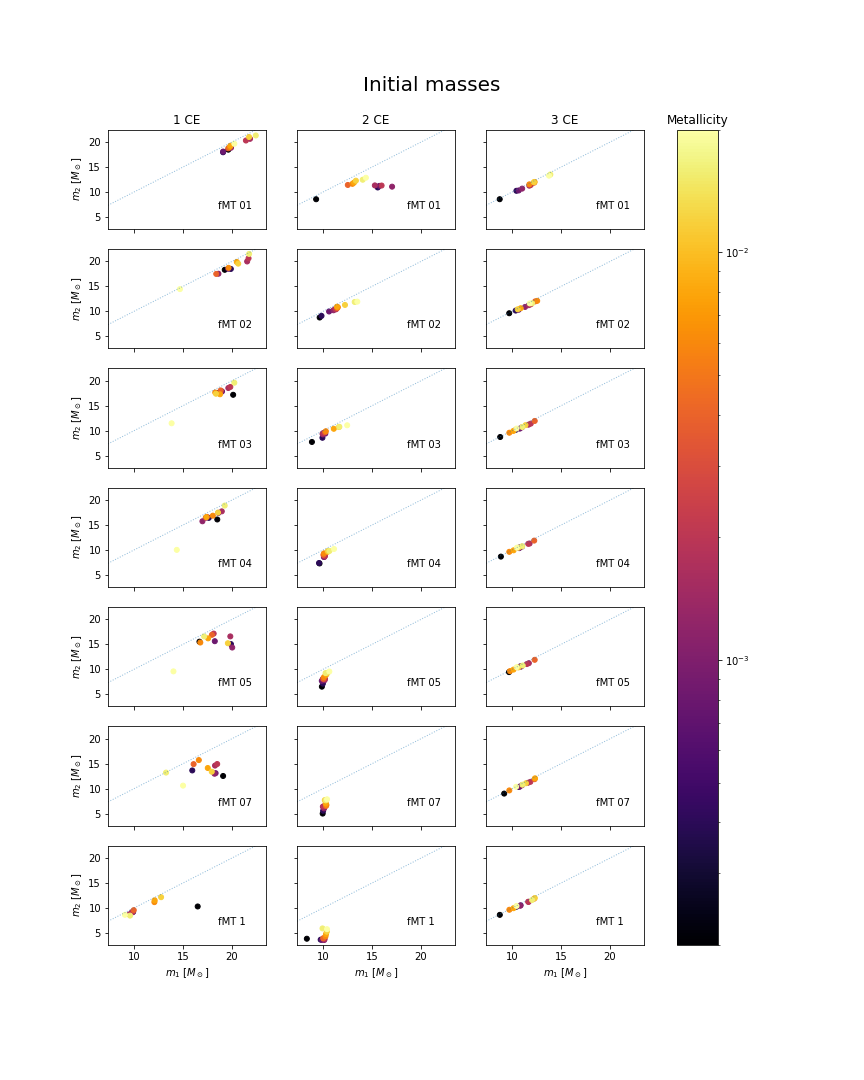
\includegraphics[width=1\textwidth]{Images/center_densities_initial.png}
    \caption{Curves describing the coordinates of densest bins, in terms of the masses of the progenitors $m_1$ and $m_2$. The bisector line where the two masses are equal is visible. }
    \label{img:initial_masses_densest_bin}
  \end{figure}
  
According to the Fig.\ref{img:initial_masses_densest_bin}, the most common systems going through one CE tend to have higher $m_1$ and $m_2$ compared to the other cases, while the ratio between initial masses slightly differs from 1. Moreover, points are sparser than others, and no general pattern is easily identified. This is coherent to what we have found previously in Fig.\ref{img:scatter_initial}. Note that for the mass conservative case, the most probable systems tend to cluster towards least massive ones. This may be since the resulting compact objects, being the total mass preserved, are more likely to collapse into BHs.\\

The last consideration is about the points related to three CE that lies on the bisector line (i.e., the locus of points where the two masses are equal). Higher the metallicity, the more massive the progenitors. 
\\
\begin{figure}[htp]
    \centering
    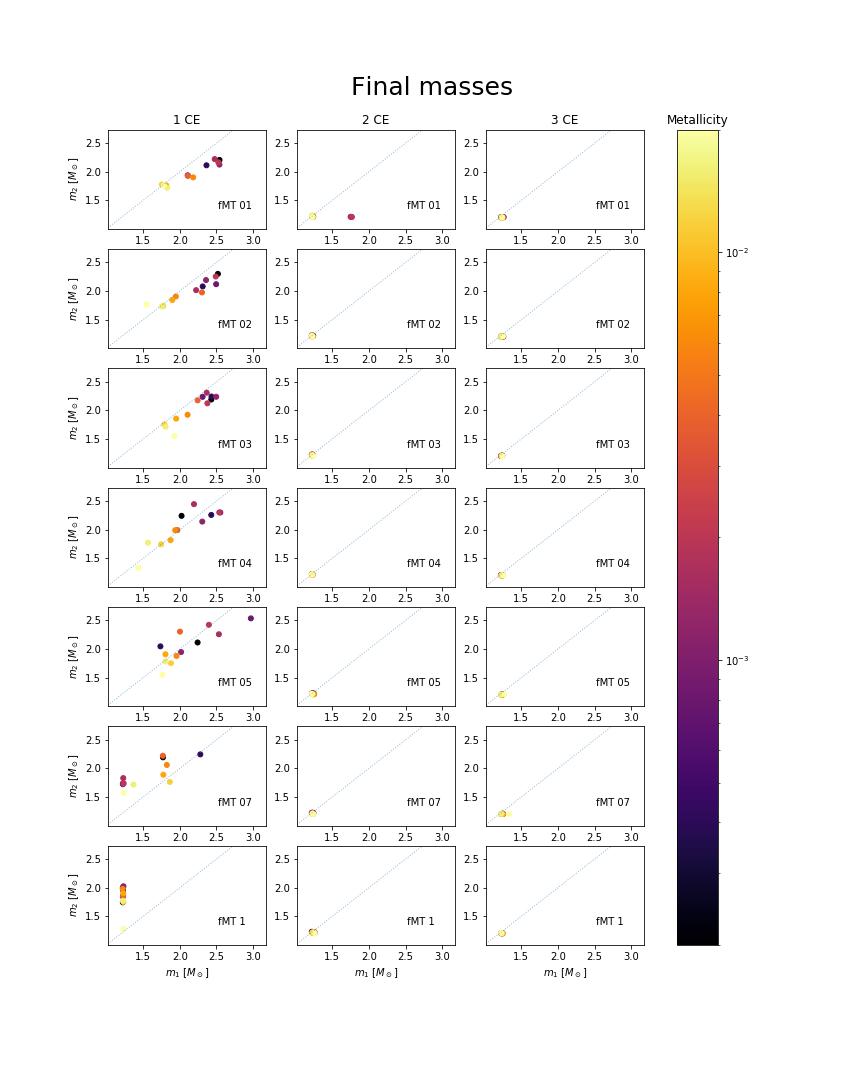
\includegraphics[width=1\textwidth]{Images/center_densities_final.png}
    \caption{Curves describing how the coordinates of densest bins, in terms of the masses of the progenitors $m_1$ and $m_2$. Bisector line where the two masses are equal is visible.}
    \label{img:final_masses_densest_bin}
  \end{figure}


Note as for final masses (Fig.\ref{img:final_masses_densest_bin}), there is no dependence on $fMT$ and $Z$ for systems that go through two and three CE, beside stochastic oscillations. For these systems, stellar winds are irrelevant, and so dependence on $Z$ and $fMT$ is lost. The same results could have been deduced also from Fig.(\ref{img:m1_zoom}) and Fig.(\ref{img:m2_zoom}). This is again an effect of Fryer prescription: the mass of NS is the result of a fit using both Carbon-Oxygen core mass and final mass of the envelope. Being the latter left behind, only the CO is usable for the fit, and that is why NS has a very well defined mass.\\

\newpage

\section{Conclusions}
In this work, we have analyzed the output of the MOBSE simulation, primarily focused on the binary systems which might evolve into NS. Taking into account the fraction of merging systems with respect to the total number, we have noticed that the number of systems that merge is dependent on $Z$ and $fMT$ (Fig.\ref{img:merging_vs_Z}). In the future, we shall investigate the merging fraction of binary NS-BH systems and its behavior for $fMT$ and $Z$ and compare it with BNSs.\\

Further, we have considered only systems that merge within a Hubble time and plotted the difference in mass units between progenitor masses, and the COs formed (Fig.\ref{img:ZAMS_vs_NS}) to discover the possibility of high massive progenitors ending up as BNSs. Interestingly, preliminary histogram analysis of the distribution of masses for both the NS that would form, we have spotted the presence of the NS formation by the process of electron capture supernovae (Fig.\ref{img:m1_zoom}).\\ 

In addition, we have understood how the density plots for delay times follow, in $log-log$ scale, a linear law (Fig.\ref{img:a_coefficient_first}) and computed the slope of the latter. Later, we considered systems by grouping them by number and type (Sec.\ref{sec:type_CE}) of CEs they go through. The delay times power-law coefficient has been computed as well by distinguishing systems based on the number of CE they go through.\\

Finally, we have considered both the masses of the progenitors by grouping them by the number of CE and the compact objects they would form (Fig.\ref{img:scatter_plots}). The density and the coordinates are plotted, in terms of $m_1$ and $m_2$, of the densest bin (Fig.\ref{img:initial_masses_densest_bin}, \ref{img:final_masses_densest_bin}). The nature of these plots is to be studied in the future.




%% The Appensuldices part is started with the command \appendix;
%% appendix sections are then done as normal sections
%% \appendix

%% \section{}
%% \label{}

%% References
%%
%% Following citation commands can be used in the body text:
%% Usage of \cite is as follows:
%%   \cite{key}          ==>>  [#]
%%   \cite[chap. 2]{key} ==>>  [#, chap. 2]
%%   \citet{key}         ==>>  Author [#]

%% References with bibTeX database:

% \bibliographystyle{model1-num-names}

%% New version of the num-names style
\newpage

\bibliographystyle{elsarticle-num-names}
\bibliography{sample.bib}

%% Authors are advised to submit their bibtex database files. They are
%% requested to list a bibtex style file in the manuscript if they do
%% not want to use model1-num-names.bst.

%% References without bibTeX database:

% \begin{thebibliography}{00}

%% \bibitem must have the following form:
%%   \bibitem{key}...
%%

% \bibitem{}

% \end{thebibliography}


\end{document}

%%
%% End of file `elsarticle-template-1-num.tex'.